% =====================================================================
%  Tracing Policy Priorities in Nepal: A Comparative Topic Modeling
%  Analysis of Government Five-Year Plans and Budget Speeches
%
%  IEEE Conference style, two-column.  Compile with pdflatex or via
%  Overleaf (template: IEEE Conference Template).  Place all PNGs from
%  ../figures/ next to this .tex file before compiling, or point
%  \graphicspath{} to that folder (already done below).
% =====================================================================
\documentclass[conference]{IEEEtran}
\IEEEoverridecommandlockouts

\usepackage{cite}
\usepackage{amsmath,amssymb,amsfonts}
\usepackage{algorithmic}
\usepackage{graphicx}
\usepackage{textcomp}
\usepackage{xcolor}
\usepackage{booktabs}
\usepackage{url}
\usepackage{caption}
\usepackage{hyperref}
\usepackage{listings}

\graphicspath{{../figures/}{./figures/}{./}}

% Listing style for the code appendix (Python).
\lstdefinestyle{pycode}{
  language=Python,
  basicstyle=\ttfamily\scriptsize,
  keywordstyle=\color{blue!60!black},
  commentstyle=\color{green!45!black}\itshape,
  stringstyle=\color{red!55!black},
  numbers=left, numberstyle=\tiny\color{gray}, numbersep=5pt,
  showstringspaces=false, breaklines=true, breakatwhitespace=false,
  frame=single, rulecolor=\color{gray!40}, tabsize=4,
  columns=fullflexible, keepspaces=true, upquote=true,
}

\def\BibTeX{{\rm B\kern-.05em{\sc i\kern-.025em b}\kern-.08em
    T\kern-.1667em\lower.7ex\hbox{E}\kern-.125emX}}

\begin{document}

\title{Tracing Policy Priorities in Nepal:\\
A Comparative Topic Modeling Analysis of Government Five-Year Plans and Budget Speeches}

\author{
\IEEEauthorblockN{Sandesh Tamang}
\IEEEauthorblockA{Softwarica College of IT and E-Commerce\\
in collaboration with Coventry University\\
Kathmandu, Nepal}
\and
\IEEEauthorblockN{Aishwarya Rai}
\IEEEauthorblockA{Softwarica College of IT and E-Commerce\\
in collaboration with Coventry University\\
Kathmandu, Nepal}
}

\maketitle

% --------------------------------------------------------------------
\begin{abstract}
We examine seventeen years of Nepali development discourse by combining
\emph{Latent Dirichlet Allocation} (LDA) with a \emph{Gaussian Process}
(GP) classifier and regressor.  A corpus of three Periodic Plans
published by the National Planning Commission (2007--2024) and eight
annual budget speeches delivered by the Ministry of Finance is split
into 345 fixed-length chunks and modelled with eight latent topics.
The discovered themes -- fiscal management, macroeconomic policy,
trade and industry, infrastructure, human development, governance,
agriculture, and federal allocation -- align closely with the
substantive content of Nepal's planning literature.  Using the
per-chunk topic distributions as features, a GP classifier with an
RBF kernel separates Plans from Budget Speeches at $90.7\% \pm 2.8\%$
five-fold cross-validated accuracy, exceeding a logistic-regression
baseline by roughly nine accuracy points.  A GP regressor with a
Mat\'ern-2.5 kernel further predicts the year of authorship to within
3.48 years on average ($R^{2}=0.353$), exposing measurable thematic
drift over the federal-transition period.  Thresholding this
continuous year output at the 2015 constitutional transition yields a
binary era label on which the GP classifier reaches
$72.8\%\pm6.2\%$ accuracy -- statistically level with a logistic
baseline -- confirming that the drift is real but gradual rather than
abrupt.  The study illustrates how
unsupervised text mining and probabilistic supervised models can be
combined to quantify policy continuity and change in a
low-resource governance setting, and it releases a reproducible
pipeline for follow-up work.
\end{abstract}

\begin{IEEEkeywords}
Topic modelling, Latent Dirichlet Allocation, Gaussian Process,
text mining, public policy, Nepal, budget speech, periodic plan.
\end{IEEEkeywords}

% --------------------------------------------------------------------
\section{Introduction}
Periodic Plans and annual budget speeches are the two flagship texts
through which the Government of Nepal communicates its development
intent.  Periodic Plans, published every three to five years by the
National Planning Commission, set medium-term sectoral targets, while
budget speeches operationalise those targets through fiscal-year
allocations announced by the Minister of Finance.  Together they form
a long, dense and surprisingly under-analysed record of the country's
policy priorities -- a record that spans monarchy, civil conflict,
constitutional change and the on-going federal transition.

Most existing scholarship on Nepal's plans is qualitative and relies
on close-reading of individual documents.  Quantitative comparative
work is rare, partly because the documents are long (the
Fifteenth Plan alone exceeds 180{,}000 words) and partly because they
are scattered across several ministry portals in heterogeneous
formats.  In this paper we treat the corpus as a single textual data
set and ask three questions:

\begin{enumerate}
\item Which latent themes recur across plans and speeches, and in what
      proportions?
\item Can a probabilistic supervised model decide, from theme
      composition alone, whether an unseen passage came from a Plan or
      from a Budget Speech?
\item Do the thematic mixtures themselves carry a temporal signature
      strong enough to date a passage?
\end{enumerate}

We answer the first question with Latent Dirichlet Allocation
(LDA)~\cite{blei2003latent}, the second with a Gaussian Process (GP)
classifier~\cite{rasmussen2006gaussian} on the per-document topic
distributions, and the third with a GP regressor whose kernel encodes
smoothness assumptions appropriate for a slowly evolving discourse; a
fourth experiment thresholds the regression target into eras and
classifies them, directly addressing the temporal question as a
decision problem.

% --------------------------------------------------------------------
\section{Related Work}\label{sec:related}
Topic modelling is widely applied to legislative and budgetary text.
Quinn~\textit{et al.}~\cite{quinn2010} track U.S.\ Senate attention
with a dynamic topic model; Grimmer and Stewart~\cite{grimmer2013text}
survey the field; Lucas~\textit{et al.}~\cite{lucas2015computer}
extend it to multilingual political corpora; and work on World Bank
narratives~\cite{moretti2015} shows latent themes can be tracked
through time even in highly formulaic genres.  For Nepal the
quantitative literature is sparse and largely hand-coded; to our
knowledge no study has combined LDA with a Gaussian Process layer on
the periodic-plan/budget-speech corpus.

GPs suit this regime: the post-LDA input is low-dimensional (eight
topics), the training set is modest (a few hundred chunks), and the
posterior gives calibrated uncertainty alongside a point
prediction~\cite{rasmussen2006gaussian,williams1998bayesian}.  RBF and
Mat\'ern kernels supply contrasting smoothness priors, useful when
prior beliefs about the feature geometry are
weak~\cite{stein1999interpolation}.

% --------------------------------------------------------------------
\section{Problem and Data Set}\label{sec:data}

\subsection{Documents collected}
Three Periodic Plans (Eleventh Three-Year Interim Plan 2007/08--2009/10,
Thirteenth Plan 2013/14--2015/16, and Fifteenth Plan
2019/20--2023/24~\cite{npc15}) were downloaded in their official English versions
from the National Planning Commission and from public mirrors
maintained by ICIMOD, the Asian Development Bank, and FAOLEX.  Eight
budget speeches covering fiscal years 2008/09 through
2024/25~\cite{mof2024} were
downloaded from the Ministry of Finance archive
(\texttt{mof.gov.np}) and verified against alternative mirrors when
the primary link returned an HTTP error.  Table~\ref{tab:corpus}
summarises the collected material.

\begin{table}[t]
\caption{Source documents in the corpus.}
\label{tab:corpus}
\centering
\small
\begin{tabular}{lcr}
\toprule
Document & Year & Words \\ \midrule
11th Three-Year Interim Plan & 2007 & 177{,}025 \\
13th Plan, Approach Paper    & 2013 &  58{,}296 \\
15th Periodic Plan           & 2019 & 186{,}314 \\ \midrule
Budget Speech FY2008/09      & 2008 &  40{,}195 \\
Budget Speech FY2014/15      & 2014 &  36{,}718 \\
Budget Speech FY2016/17      & 2016 &  43{,}302 \\
Budget Speech FY2017/18      & 2017 &  38{,}626 \\
Budget Speech FY2018/19      & 2018 &  24{,}632 \\
Budget Speech FY2021/22      & 2021 &  38{,}390 \\
Budget Speech FY2023/24      & 2023 &  24{,}005 \\
Budget Speech FY2024/25      & 2024 &  17{,}441 \\ \midrule
\textbf{Total}               &      & \textbf{684{,}944} \\
\bottomrule
\end{tabular}
\end{table}

\subsection{Why these documents matter}
The window straddles three regimes that should leave thematic
fingerprints: the post-conflict transitional government (2007--2014),
the 2015 Constitution and move to federalism (2015--2017), and
consolidation under Province governments (2018--2024).  Whether a
method can separate these regimes from internal language alone is
therefore informative either way.

\subsection{Pre-processing}
The documents are PDFs, so we use \texttt{pypdf} to extract raw
character streams, re-join hyphenated line breaks, collapse repeated
whitespace, and cast everything to lower case.  Each cleaned document
is partitioned into non-overlapping chunks of $\sim$2{,}000 words to
expose enough units (345 in total) for stable variational inference.
Tokens are extracted with the regular expression
\verb|[a-z]{3,}|, the NLTK English stopword list is applied, and a
manually-curated list of 70 boilerplate terms specific to Nepali
government English (\textit{nepal}, \textit{government},
\textit{ministry}, \textit{fiscal}, \textit{rupees}, \dots) is removed
so that they do not dominate the topics.  The resulting vocabulary
has 4{,}000 terms after enforcing $\min\!=\!3$ document frequency and
$\max\!=\!0.85$ document frequency.

% --------------------------------------------------------------------
\section{Methods}\label{sec:methods}

\subsection{Latent Dirichlet Allocation}
LDA models each document $d$ as a mixture over $K$ latent topics
$\theta_d \sim \operatorname{Dir}(\alpha)$ and each topic $k$ as a
distribution over the vocabulary
$\phi_k \sim \operatorname{Dir}(\beta)$.  A token $w_{dn}$ is generated
by first drawing a topic $z_{dn}\!\sim\!\operatorname{Cat}(\theta_d)$
and then a word $w_{dn}\!\sim\!\operatorname{Cat}(\phi_{z_{dn}})$.  We
fit LDA with batch variational Bayes as implemented in
\texttt{scikit-learn}, using $\alpha=0.1$ (favouring sparse
document-topic mixtures) and $\beta=0.01$ (favouring sparse
topic-word distributions), 40 outer iterations and a fixed random
seed.

\subsection{Gaussian Process classifier}
After LDA we obtain a feature matrix
$\Theta \in \mathbb{R}^{N\times K}$, where $\Theta_{d,k}$ is the
expected proportion of topic $k$ in chunk $d$.  We model the binary
label $y_d \in\{\text{plan},\text{speech}\}$ with a GP classifier
whose latent function $f$ has prior
$f \sim \operatorname{GP}(0, k(\cdot, \cdot))$ and likelihood
$p(y\!\mid\! f)=\Phi(yf)$.  The kernel used is
\begin{equation}
k(x,x') \;=\; \sigma_{f}^{2}\,
              \exp\!\Bigl(-\tfrac{\|x-x'\|^{2}}{2\ell^{2}}\Bigr)
              \;+\; \sigma_{n}^{2}\,\delta_{xx'},
\end{equation}
i.e.\ a constant-scaled RBF plus a white-noise term.  Hyperparameters
$\{\sigma_{f},\ell,\sigma_{n}\}$ are obtained by maximising the
log-marginal likelihood with two random restarts.

\subsection{Gaussian Process regressor for time}
For dating an unseen passage we regress the (continuous) year of
authorship on the same topic vector.  Because the year axis is short
($2007$--$2024$) and the underlying topic drift is expected to be
smooth but not infinitely differentiable, we adopt a Mat\'ern-2.5
kernel,
\begin{equation}
k_{\nu=5/2}(x,x') \;=\;
   \Bigl(1 + \tfrac{\sqrt{5}r}{\ell} + \tfrac{5r^{2}}{3\ell^{2}}\Bigr)
   \exp\!\Bigl(-\tfrac{\sqrt{5}r}{\ell}\Bigr),
\end{equation}
with $r=\|x-x'\|$, again coupled with an explicit white-noise term.

\subsection{Thresholded-output GP classification}
The brief asks specifically for a GP classifier trained on a class
variable obtained by \emph{thresholding} a continuous output.  We use
the document year for this purpose: applying the threshold
$\tau=2015$ -- the year Nepal promulgated its federal constitution --
maps every chunk to a binary era label
$e_d=\mathbb{1}[\text{year}_d>\tau]$ (pre-federal vs.\ federal).  The
same RBF-plus-noise kernel and optimisation procedure as the genre
classifier are then applied to $(\Theta, e)$.  Unlike the genre label,
the era label is \emph{derived} from a continuous quantity, so this
experiment tests whether the topic mixtures encode a sharp regime
boundary or only a gradual drift.

\subsection{Baselines and evaluation}
For classification we compare against $\ell_{2}$-regularised
logistic regression; for regression we compare against ridge
regression.  All models are evaluated with five-fold cross-validation,
stratified by class for the classifier and shuffled for the
regressor.  We report accuracy, macro-$F_{1}$, mean absolute error
(MAE) and $R^{2}$ together with cross-fold standard deviations.

% --------------------------------------------------------------------
\section{Experimental Setup}\label{sec:setup}
The pipeline is implemented in Python~3.12 using
\texttt{scikit-learn}~1.8~\cite{pedregosa2011}, \texttt{nltk},
\texttt{pypdf} and the usual scientific stack, managed with \texttt{uv}; a full run completes in
under four minutes on an Apple Silicon CPU, with all random seeds
fixed at $42$.

To choose the number of topics we sweep $K\!\in\!\{4,6,8,10,12\}$ and
record held-out perplexity.  Perplexity falls monotonically
(Fig.~\ref{fig:perp}), so we select $K\!=\!8$ as a compromise between
fit and interpretability; beyond eight, components fragment existing
themes or attach to surviving boilerplate.

\begin{figure}[t]
\centering
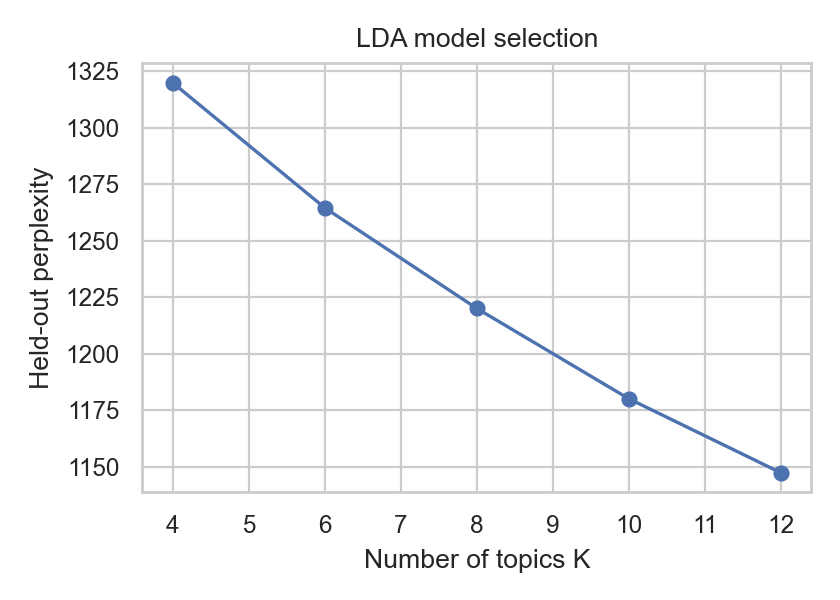
\includegraphics[width=0.85\columnwidth]{fig_perplexity.png}
\caption{Held-out perplexity as a function of the number of topics
$K$.  Perplexity falls monotonically but with diminishing returns;
$K\!=\!8$ is chosen for interpretability.}
\label{fig:perp}
\end{figure}

% --------------------------------------------------------------------
\section{Results}\label{sec:results}

\subsection{Discovered topics}
Table~\ref{tab:topics} lists the eight highest-probability terms for
each topic and Fig.~\ref{fig:wordcloud} shows the corresponding
word-clouds.  The themes are readily recognisable to a reader of
Nepali planning discourse: T1 fiscal accounts, T2 macroeconomy, T3
trade/energy/provinces, T4 infrastructure, T5 human development, T6
implementation and governance, T7 agriculture and land, and T8 the
federal financial structure (recurrent/capital splits, Federal
Affairs, the Auditor-General).  T8 is the most diagnostic: as
Section~\ref{sec:results} shows, it barely existed before the 2015
federal transition.

\begin{table*}[t]
\caption{Top eight words for each LDA topic ($K=8$).}
\label{tab:topics}
\centering
\small
\begin{tabular}{ll}
\toprule
Topic & Top words \\ \midrule
T1 (Fiscal)        & tax, grant, revenue, capital, loan, expenditure, foreign, expenses \\
T2 (Macroeconomy)  & economic, investment, foreign, growth, rate, financial, increase, sectors \\
T3 (Trade/Energy)  & energy, tourism, goods, trade, province, export, industrial, supply \\
T4 (Infrastructure)& construction, project, road, water, infrastructure, electricity, completed, transport \\
T5 (Human dev.)    & health, education, social, women, human, security, rights, children \\
T6 (Governance)    & programs, system, implementation, monitoring, rural, evaluation, projects, service \\
T7 (Agriculture)   & land, agriculture, production, food, agricultural, irrigation, forest, areas \\
T8 (Federal fin.)  & capital, recurrent, financing, affairs, commission, federal, finance, education \\
\bottomrule
\end{tabular}
\end{table*}

\begin{figure}[t]
\centering

\includegraphics[width=\columnwidth]{fig_wordclouds.png}
\caption{Word-clouds for the eight LDA topics.  Larger words have
higher probability within the topic.}
\label{fig:wordcloud}
\end{figure}

\subsection{Plans versus budget speeches}
Fig.~\ref{fig:topic-cat} contrasts mean topic probability by genre.
Plans are dominated by T2 (macroeconomy), T5 (human development), T6
(governance) and T7 (agriculture); Speeches by T1 (fiscal accounts),
T4 (infrastructure) and T8 (federal finance) -- exactly the expected
division of labour, with Plans setting medium-term strategy in
sectoral language and Speeches announcing fiscal-year allocations in
line-item language.

\begin{figure}[t]
\centering
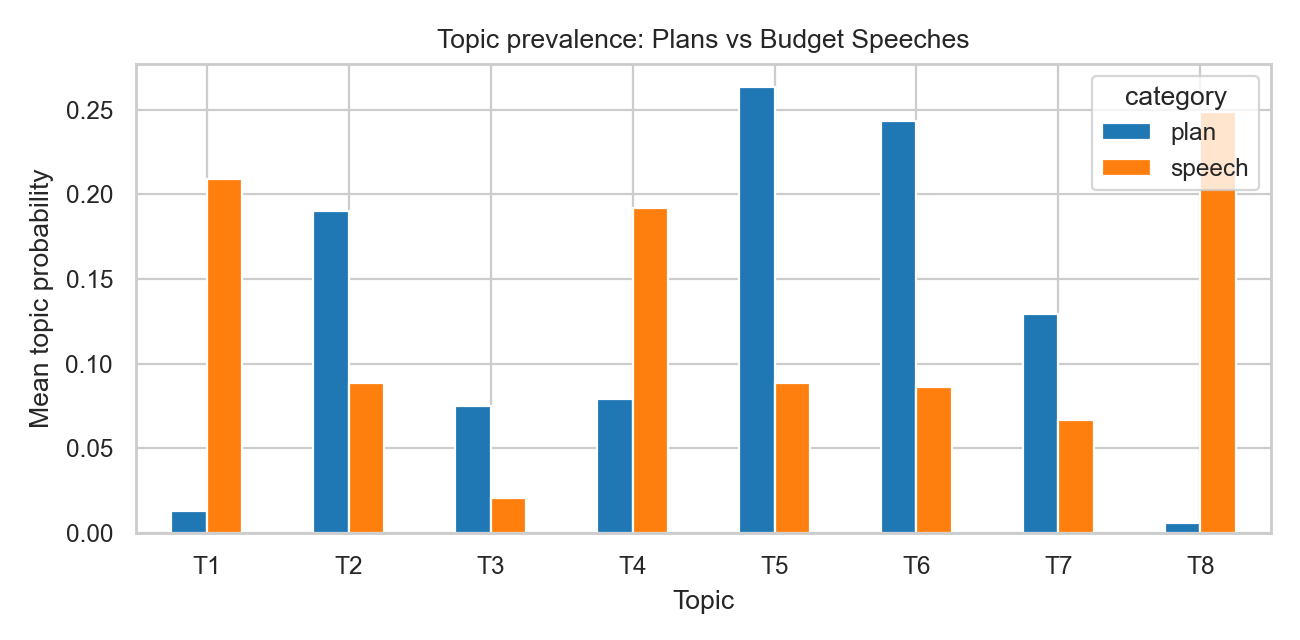
\includegraphics[width=\columnwidth]{fig_topic_category.png}
\caption{Mean topic probability per category.  Plans emphasise
sectoral and governance topics; Budget Speeches emphasise fiscal,
infrastructure and federal-finance topics.}
\label{fig:topic-cat}
\end{figure}

\subsection{Gaussian Process classification}
With these eight features the GP classifier separates the two genres
at a cross-validated accuracy of $0.907 \pm 0.028$ and macro-$F_{1}$
of $0.901$, compared with $0.820 \pm 0.025$ accuracy and $0.798$
$F_{1}$ for logistic regression on the same features
(Table~\ref{tab:cls}).  Fig.~\ref{fig:conf} shows the confusion
matrix on the full training set ($210{+}132$ correct, three errors).
The misclassified chunks turn out to belong to the macroeconomic
overview sections of budget speeches, which are written in the same
strategic register as Plans.

\begin{table}[t]
\caption{Classification of Plans vs Budget Speeches (5-fold CV).}
\label{tab:cls}
\centering
\small
\begin{tabular}{lcc}
\toprule
Model                 & Accuracy            & Macro $F_{1}$       \\ \midrule
Logistic Regression   & $0.820 \pm 0.025$   & $0.798 \pm 0.032$   \\
\textbf{GP (RBF)}     & $\mathbf{0.907 \pm 0.028}$ & $\mathbf{0.901 \pm 0.032}$ \\
\bottomrule
\end{tabular}
\end{table}

\begin{figure}[t]
\centering
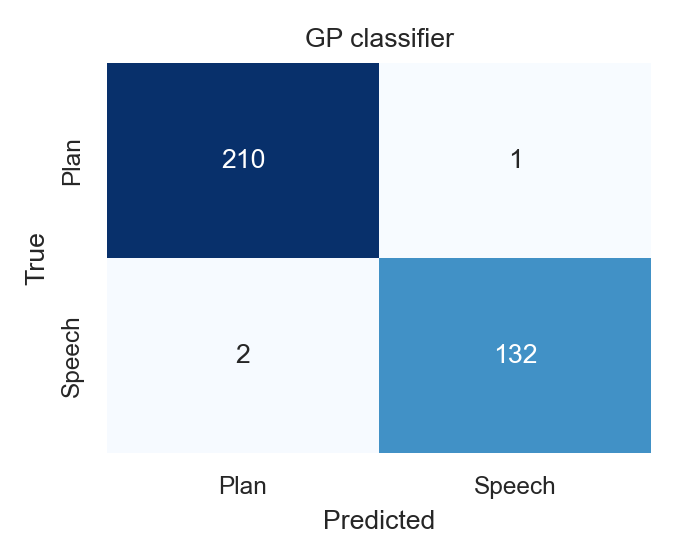
\includegraphics[width=0.7\columnwidth]{fig_confusion.png}
\caption{Confusion matrix of the GP classifier on the full corpus.}
\label{fig:conf}
\end{figure}

The t-SNE projection in Fig.~\ref{fig:tsne} provides geometric
intuition for the result: in eight-topic space the two genres
already separate into distinct clusters, leaving only a narrow
contact region for the GP decision boundary to negotiate.

\begin{figure}[t]
\centering
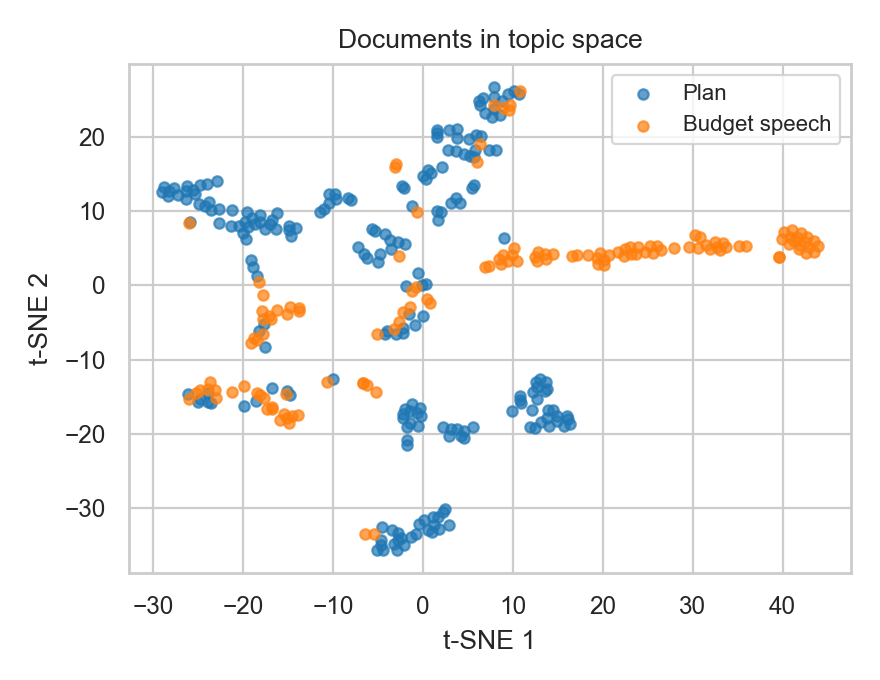
\includegraphics[width=0.85\columnwidth]{fig_tsne.png}
\caption{Two-dimensional t-SNE embedding of the per-chunk topic
distributions, coloured by document category.}
\label{fig:tsne}
\end{figure}

\subsection{Dating a passage}
Fig.~\ref{fig:time} traces the mean topic probability for each year of
the corpus.  Two qualitative observations stand out.  First, T8
(federal finance) is essentially absent before 2015 and rises sharply
after the constitution-mandated federal transition.  Second, T2
(macroeconomy) declines visibly after 2018 as the documents pivot
from aspirational growth narratives to fiscal-recovery narratives in
the COVID-19 and post-COVID years.

\begin{figure}[t]
\centering
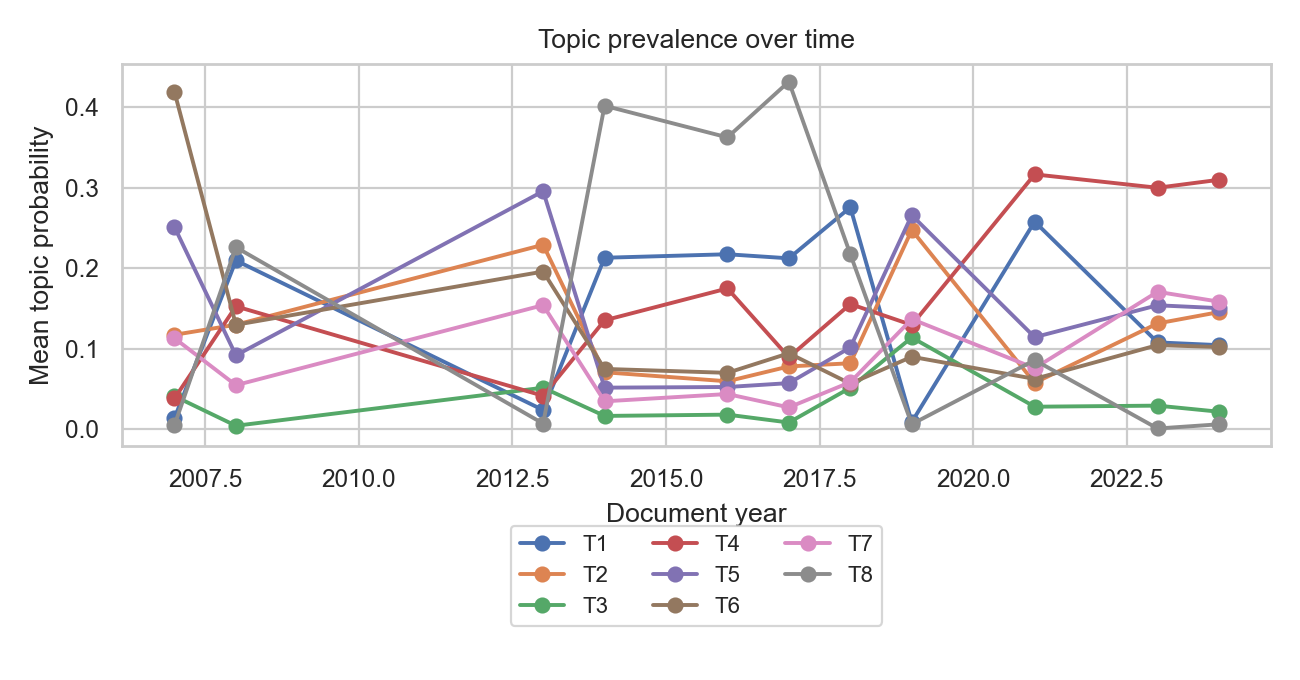
\includegraphics[width=\columnwidth]{fig_topics_over_time.png}
\caption{Mean topic probability per document year, 2007--2024.
Topic 8 (federal finance) emerges only after 2015; Topic 2
(macroeconomy) gradually loses share.}
\label{fig:time}
\end{figure}

These shifts are large enough that a GP regressor can recover the
year of a passage from its topic mixture with a cross-validated MAE
of $3.48 \pm 0.15$ years and $R^{2} = 0.353 \pm 0.138$, beating
ridge regression ($\mathrm{MAE}=3.70$, $R^{2}=0.324$) by a small but
consistent margin (Table~\ref{tab:reg}).  Fig.~\ref{fig:gpr} plots
predicted year against true year; the $\pm1\sigma$ band widens around
documents from the 2016--2017 transition years, exactly where the
discourse is most heterogeneous.

\begin{table}[t]
\caption{Year regression on topic features (5-fold CV).}
\label{tab:reg}
\centering
\small
\begin{tabular}{lcc}
\toprule
Model              & MAE (years)         & $R^{2}$              \\ \midrule
Ridge regression   & $3.70 \pm 0.12$     & $0.324 \pm 0.102$    \\
\textbf{GP (Mat\'ern-5/2)} & $\mathbf{3.48 \pm 0.15}$ & $\mathbf{0.353 \pm 0.138}$ \\
\bottomrule
\end{tabular}
\end{table}

\begin{figure}[t]
\centering
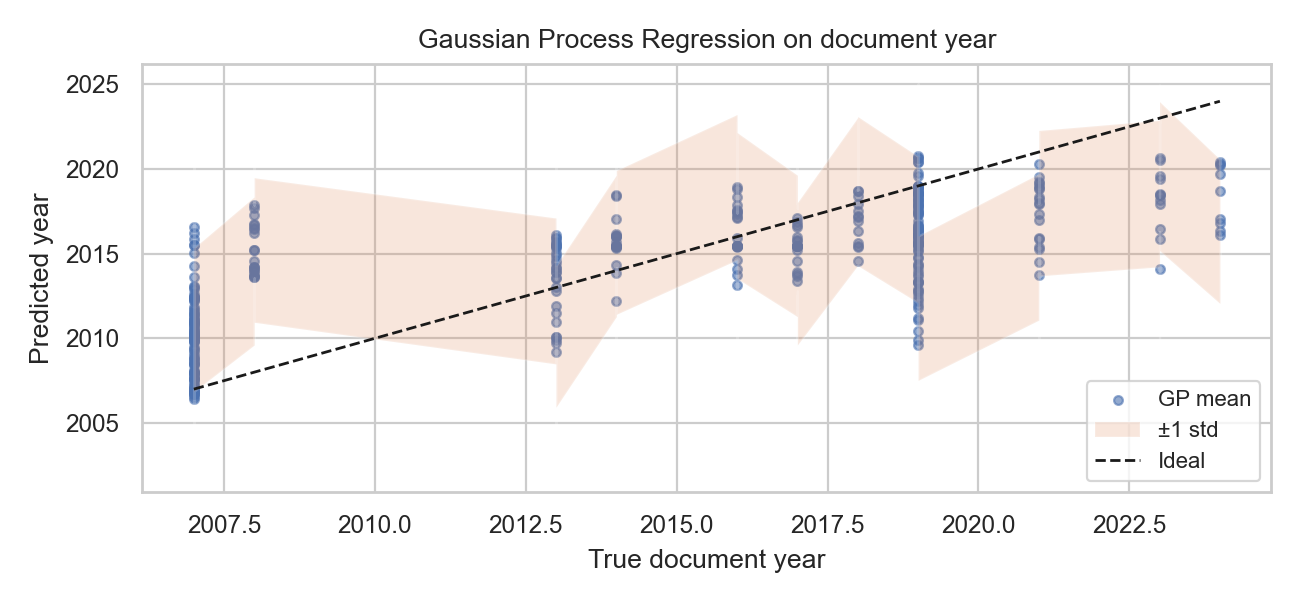
\includegraphics[width=\columnwidth]{fig_gpr_year.png}
\caption{Gaussian Process regression of document year on topic
features.  Shaded band is $\pm1\sigma$ posterior uncertainty.}
\label{fig:gpr}
\end{figure}

\subsection{Thresholding the year into eras}
Thresholding the continuous year at $\tau=2015$ splits the corpus into
157 pre-federal and 188 federal chunks and turns the dating problem
into a binary GP classification (Section~\ref{sec:methods}).  Here the
GP reaches $0.728 \pm 0.062$ accuracy and $0.716$ macro-$F_{1}$, while
logistic regression reaches $0.745 \pm 0.065$ and $0.736$
(Table~\ref{tab:era}).  Both clear the $0.545$ majority-class floor
comfortably, but their confidence intervals overlap almost entirely,
so on this task the GP offers \emph{no} advantage over the linear
model.  The confusion matrix (Fig.~\ref{fig:conf-era}) shows most
errors are pre-2015 chunks read as federal: macroeconomic and
human-development language is largely time-invariant, so only the
fiscal-structure vocabulary (T8) carries a clean date stamp.  This is
the expected counterpart to the modest regression $R^{2}$: the
2015 transition is visible in the topics but diffuse, not a step
change, which is exactly why a flexible non-linear boundary buys
nothing here.

\begin{table}[t]
\caption{Era classification from thresholded year, $\tau=2015$ (5-fold CV).}
\label{tab:era}
\centering
\small
\begin{tabular}{lcc}
\toprule
Model              & Accuracy            & Macro $F_{1}$       \\ \midrule
Majority class     & $0.545$             & ---                 \\
GP (RBF)           & $0.728 \pm 0.062$   & $0.716$             \\
Logistic Regression& $0.745 \pm 0.065$   & $0.736$             \\
\bottomrule
\end{tabular}
\end{table}

\begin{figure}[t]
\centering
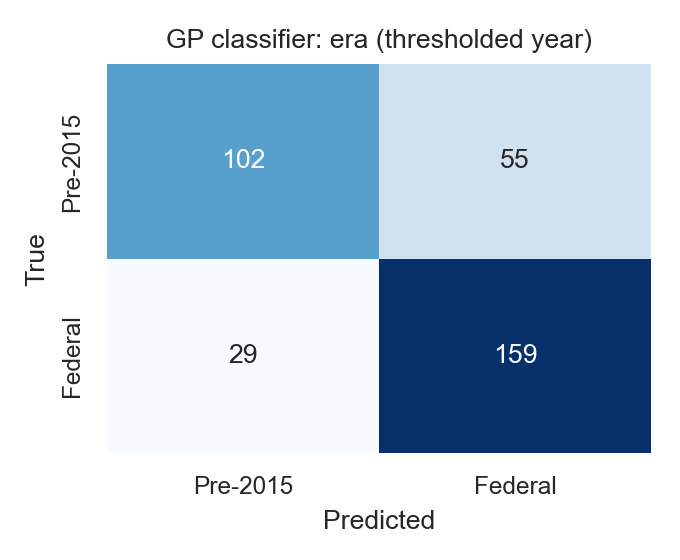
\includegraphics[width=0.7\columnwidth]{fig_confusion_era.png}
\caption{Confusion matrix of the GP era classifier (thresholded year).
Errors concentrate on pre-2015 chunks predicted as federal.}
\label{fig:conf-era}
\end{figure}

% --------------------------------------------------------------------
\section{Social, Ethical, Legal and Professional Considerations}
\label{sec:ethics}
All texts analysed are official Government of Nepal publications in
the public domain; no copyright restricts research re-use, and each
download URL is recorded in the released sources file.  Four further
considerations apply.  \emph{Representation:} a topic captures the
\emph{language} a document uses, not the \emph{adequacy} of the
allocations behind it, so any policy claim must be triangulated with
expenditure data.  \emph{Translation bias:} we use the official
English translations of the Nepali originals, and translator choices
can shift emphasis; the pipeline should ideally be re-run on the
Devanagari source with a script-aware tokeniser.  \emph{Provincial
voices:} the corpus is exclusively federal, so generalising to
``Nepali policy priorities'' \textit{tout court} would be premature.
\emph{Professional responsibility:} because the GP returns a
calibrated posterior, any oversight or journalistic deployment should
communicate uncertainty rather than headline point predictions, as
the figures here do.

% --------------------------------------------------------------------
\section{Discussion and Conclusions}\label{sec:discussion}
Combining LDA with a Gaussian Process classifier exposes a clean
quantitative distinction between Nepal's medium-term Plans and its
annual Budget Speeches: a small, well-regularised GP recovers the
distinction at $90.7\%$ accuracy from only eight latent features.
A Mat\'ern-kernel GP regressor further confirms that the corpus has a
non-trivial temporal signature -- the topics shift in measurable ways
across the constitutional and federal transitions of 2015--2018.

The GP clearly outperforms the linear baselines on the two tasks with
sharp class structure -- genre classification and year regression --
but is statistically level with logistic regression once the year is
thresholded into eras, where the boundary is diffuse.  Reporting this
null result is deliberate: the value of the GP is not a uniform
accuracy gain but its calibrated posterior, which widens for passages
near the 2015 transition -- exactly the behaviour we want from an
honest model in a regime change, and the same reason the era boundary
resists a hard decision rule.

\emph{Limitations.}  Three plans and eight speeches are a thin slice
of Nepal's planning history; extending the corpus to all sixteen
Periodic Plans and to provincial budgets would strengthen every
conclusion.  Pre-processing in English loses lexical signal that the
Nepali originals contain.  Finally, LDA assumes exchangeable bags of
words and therefore cannot capture argument structure.

\emph{Future work.}  We see two natural extensions.  First,
substituting a dynamic topic model~\cite{blei2006dynamic} for static
LDA would let topic-word distributions themselves evolve through
time.  Second, the GP classifier could be re-used as an auditing tool
for new budget speeches: a draft that scores as an outlier under the
model is, by construction, breaking with the recent fiscal rhetoric
and would warrant a closer human read.

% --------------------------------------------------------------------
\section*{Author Contributions}
The two authors contributed jointly to problem formulation, corpus
curation, and writing.  Specific contributions are as follows.
\textbf{Sandesh Tamang} led the data-engineering work (PDF
acquisition, text extraction, cleaning) and implemented the LDA
component as the shared methodology.  \textbf{Aishwarya Rai} led the
probabilistic-modelling work, implementing both the Gaussian Process
classifier on topic features and the Gaussian Process regressor for
the temporal analysis as the individual technique, and produced the
figures.  Both authors jointly wrote the manuscript and reviewed the
final results.

% --------------------------------------------------------------------
\section*{Reproducibility}
The complete pipeline -- download script, text extractor and analysis
script -- is listed in Appendix~\ref{app:code} and released at
\url{https://github.com/aishwaryawambule/policy-topic-modeling}.
Random seeds are fixed at $42$; running \texttt{01\_download.py},
\texttt{02\_extract.py} and \texttt{03\_analyze.py} in sequence
regenerates every figure and the \texttt{metrics.json} from which all
numbers above are drawn.

% --------------------------------------------------------------------
\begin{thebibliography}{99}
\bibitem{blei2003latent} D.~M. Blei, A.~Y. Ng, and M.~I. Jordan,
``Latent Dirichlet allocation,'' \emph{Journal of Machine Learning
Research}, vol.~3, pp.~993--1022, 2003.

\bibitem{rasmussen2006gaussian} C.~E. Rasmussen and C.~K.~I. Williams,
\emph{Gaussian Processes for Machine Learning}. MIT Press, 2006.

\bibitem{quinn2010} K.~M. Quinn, B.~L. Monroe, M.~Colaresi,
M.~H. Crespin, and D.~R. Radev, ``How to analyze political attention
with minimal assumptions and costs,'' \emph{American Journal of
Political Science}, vol.~54, no.~1, pp.~209--228, 2010.

\bibitem{grimmer2013text} J.~Grimmer and B.~M. Stewart, ``Text as
data: the promise and pitfalls of automatic content analysis methods
for political texts,'' \emph{Political Analysis}, vol.~21, no.~3,
pp.~267--297, 2013.

\bibitem{lucas2015computer} C.~Lucas, R.~A. Nielsen, M.~E. Roberts,
B.~M. Stewart, A.~Storer, and D.~Tingley, ``Computer-assisted text
analysis for comparative politics,'' \emph{Political Analysis},
vol.~23, no.~2, pp.~254--277, 2015.

\bibitem{moretti2015} F.~Moretti and D.~Pestre, ``Bankspeak: the
language of World Bank reports, 1946--2012,'' \emph{New Left Review},
vol.~92, pp.~75--99, 2015.

\bibitem{williams1998bayesian} C.~K.~I. Williams and D.~Barber,
``Bayesian classification with Gaussian processes,'' \emph{IEEE
Transactions on Pattern Analysis and Machine Intelligence}, vol.~20,
no.~12, pp.~1342--1351, 1998.

\bibitem{stein1999interpolation} M.~L. Stein,
\emph{Interpolation of Spatial Data: Some Theory for Kriging}.
Springer, 1999.

\bibitem{blei2006dynamic} D.~M. Blei and J.~D. Lafferty, ``Dynamic
topic models,'' in \emph{Proc.\ ICML}, 2006, pp.~113--120.

\bibitem{pedregosa2011} F.~Pedregosa \textit{et al.},
``Scikit-learn: machine learning in Python,'' \emph{Journal of
Machine Learning Research}, vol.~12, pp.~2825--2830, 2011.

\bibitem{npc15} National Planning Commission, Government of Nepal,
\emph{The Fifteenth Plan, Fiscal Year 2019/20--2023/24}.
Kathmandu: NPC, 2020. [Online].

\bibitem{mof2024} Ministry of Finance, Government of Nepal,
\emph{Budget Speech of Fiscal Year 2024/25}.  Kathmandu: MoF, 2024.
[Online].
\end{thebibliography}

\onecolumn
\appendices
\section{Source Code}\label{app:code}
The screenshots below show the three Python scripts that implement the pipeline, displayed with headings per script. The complete original text of all code is available in the project repository at \url{https://github.com/aishwaryawambule/policy-topic-modeling}; all random seeds are fixed at 42, so running the scripts in order regenerates every figure, table and number reported above.
\subsection{\texttt{01\_download.py} --- Data acquisition (downloads the source PDFs)}
\par\medskip\noindent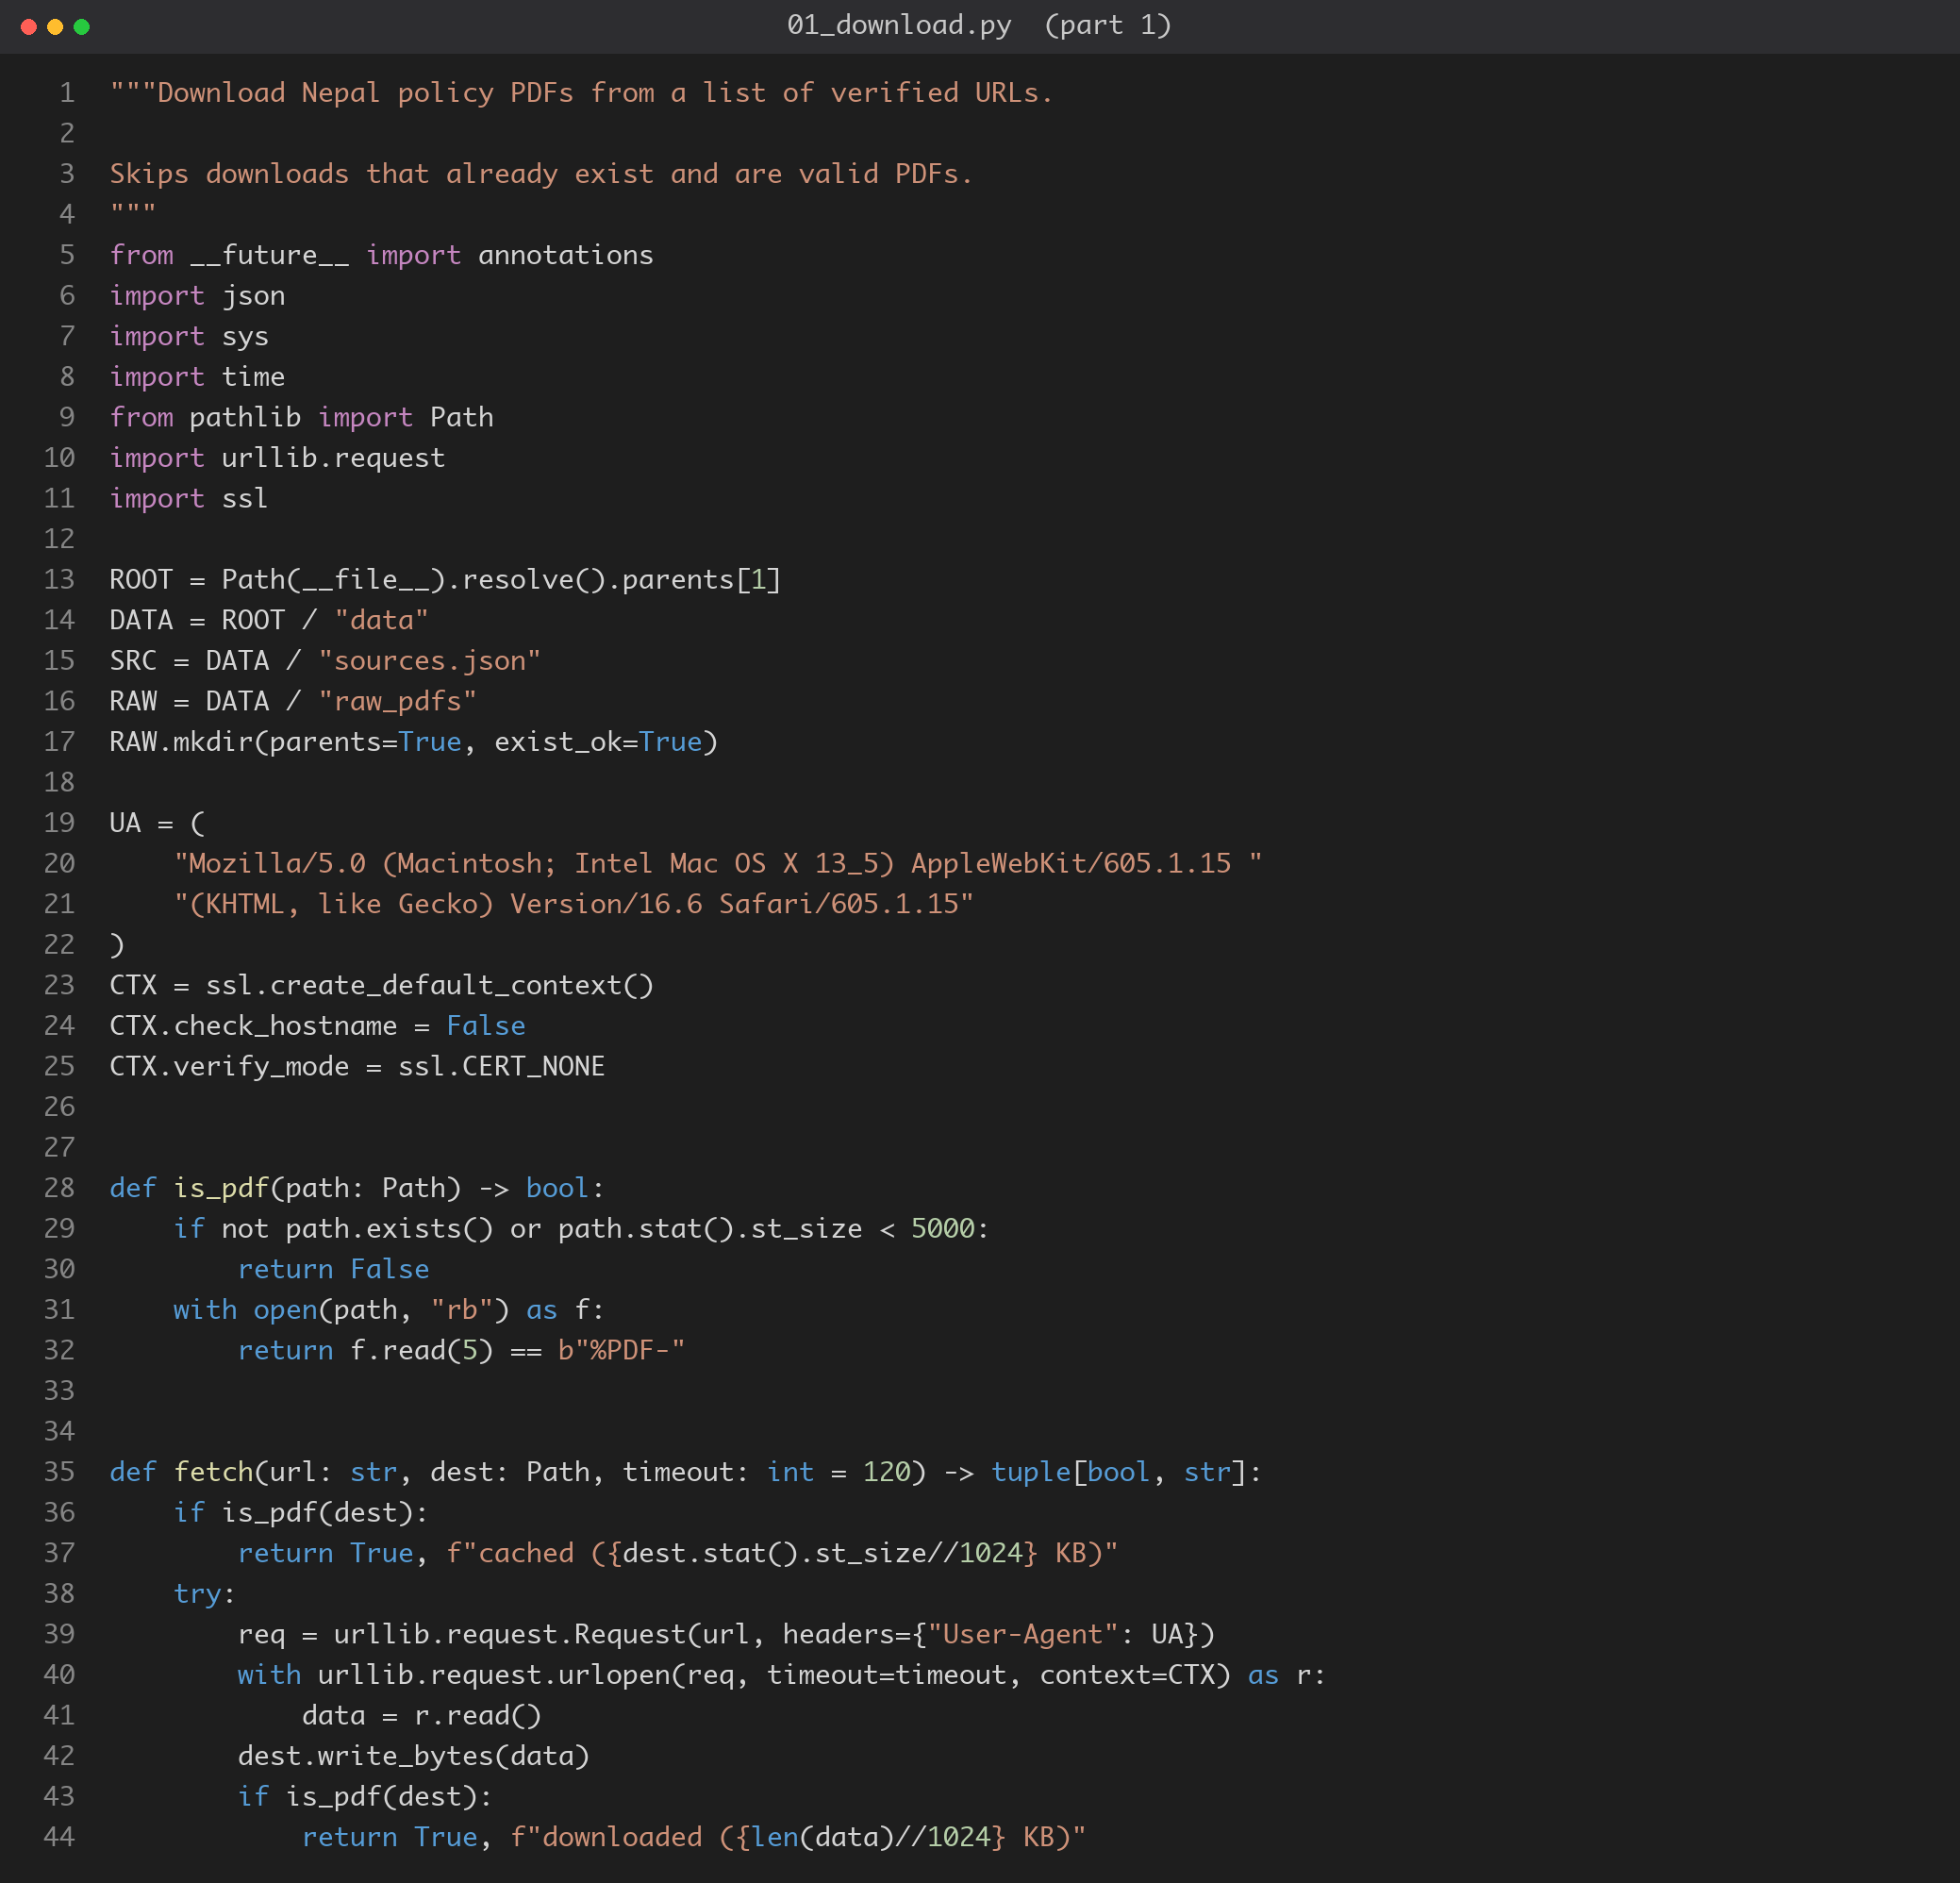
\includegraphics[width=\linewidth]{code_shots/01_download_py_p1.png}
\par\medskip\noindent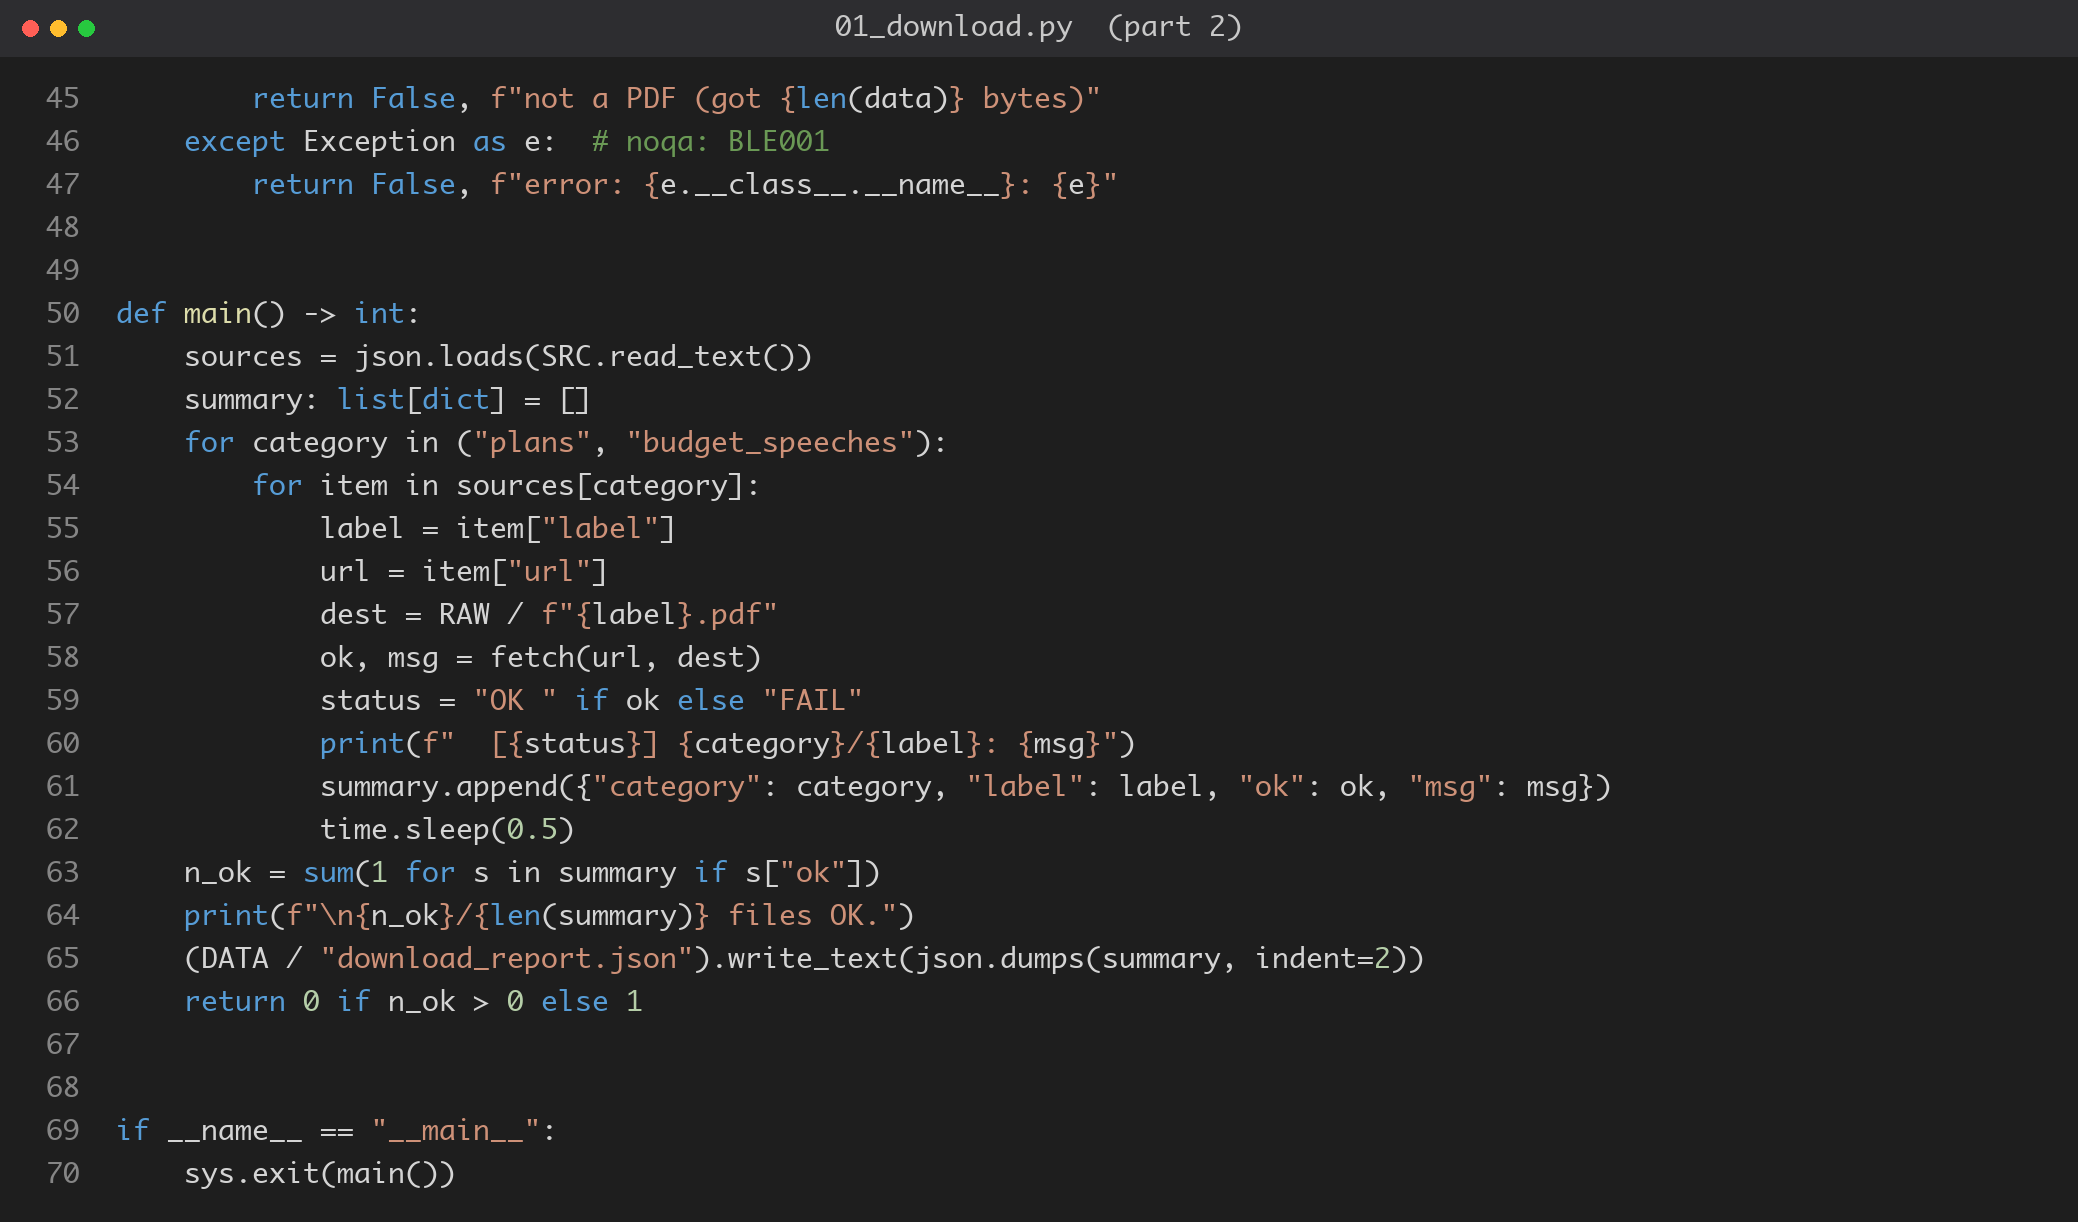
\includegraphics[width=\linewidth]{code_shots/01_download_py_p2.png}
\subsection{\texttt{02\_extract.py} --- PDF $\rightarrow$ plain-text extraction}
\par\medskip\noindent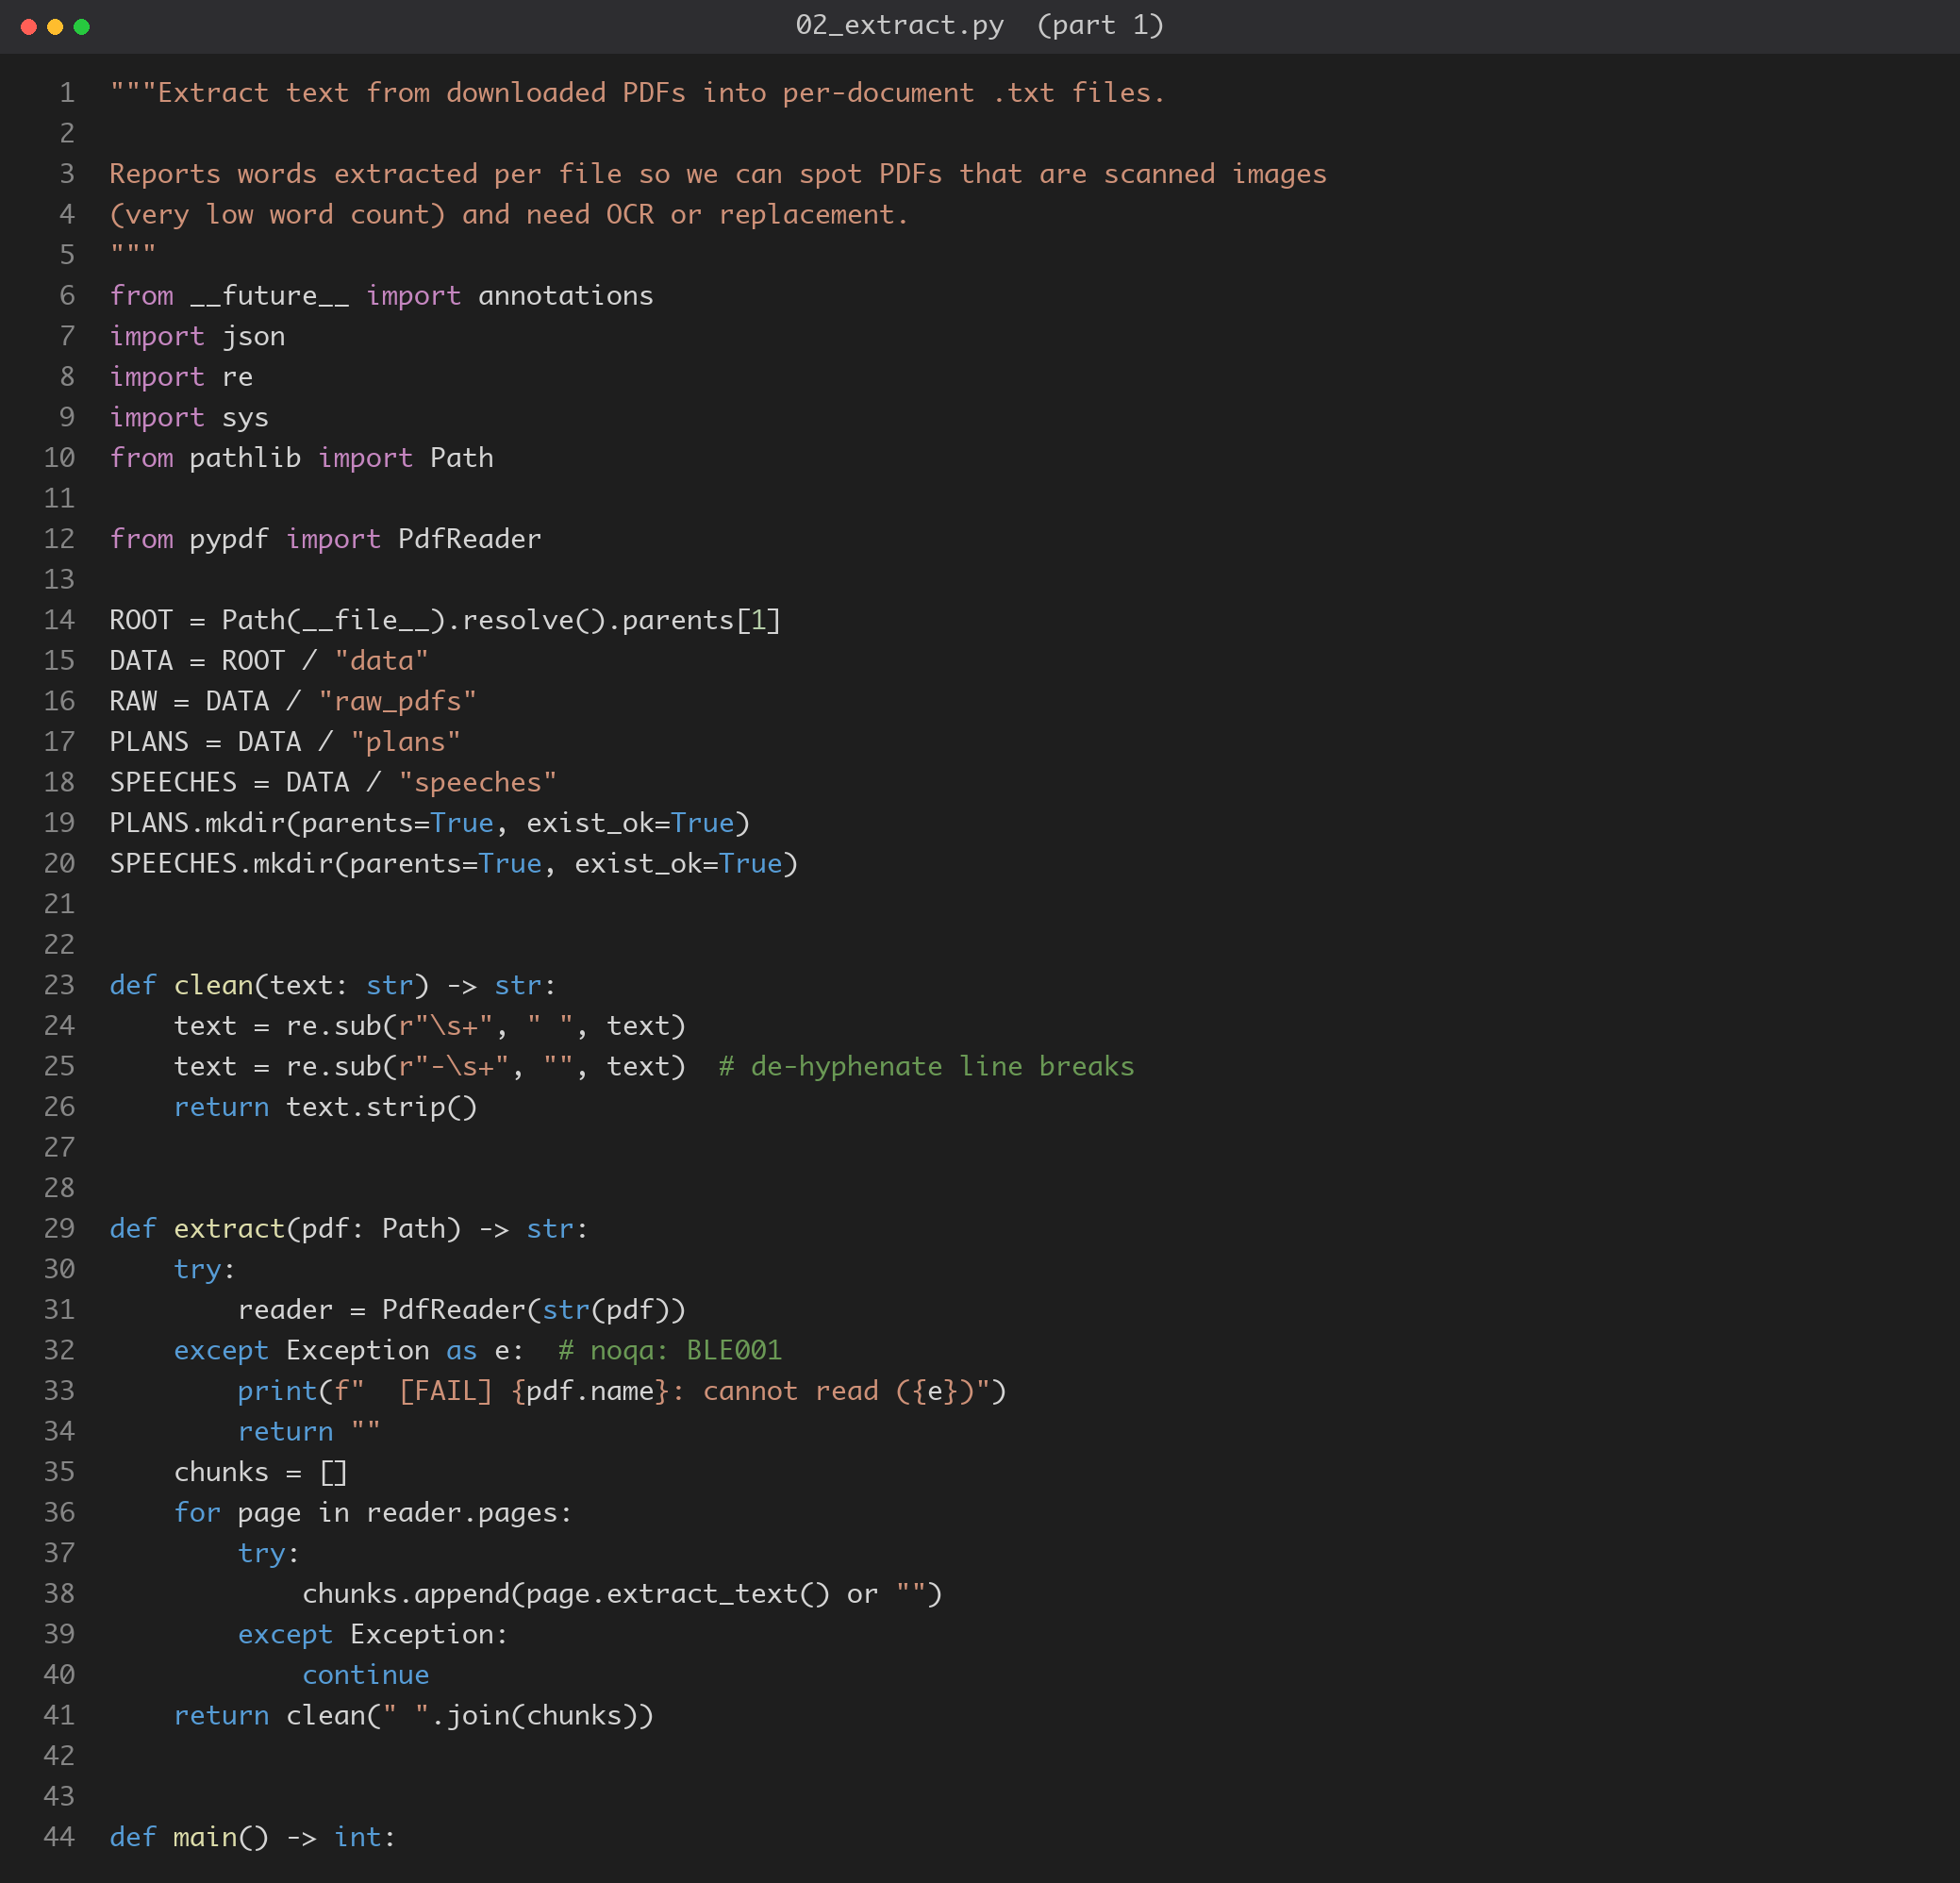
\includegraphics[width=\linewidth]{code_shots/02_extract_py_p1.png}
\par\medskip\noindent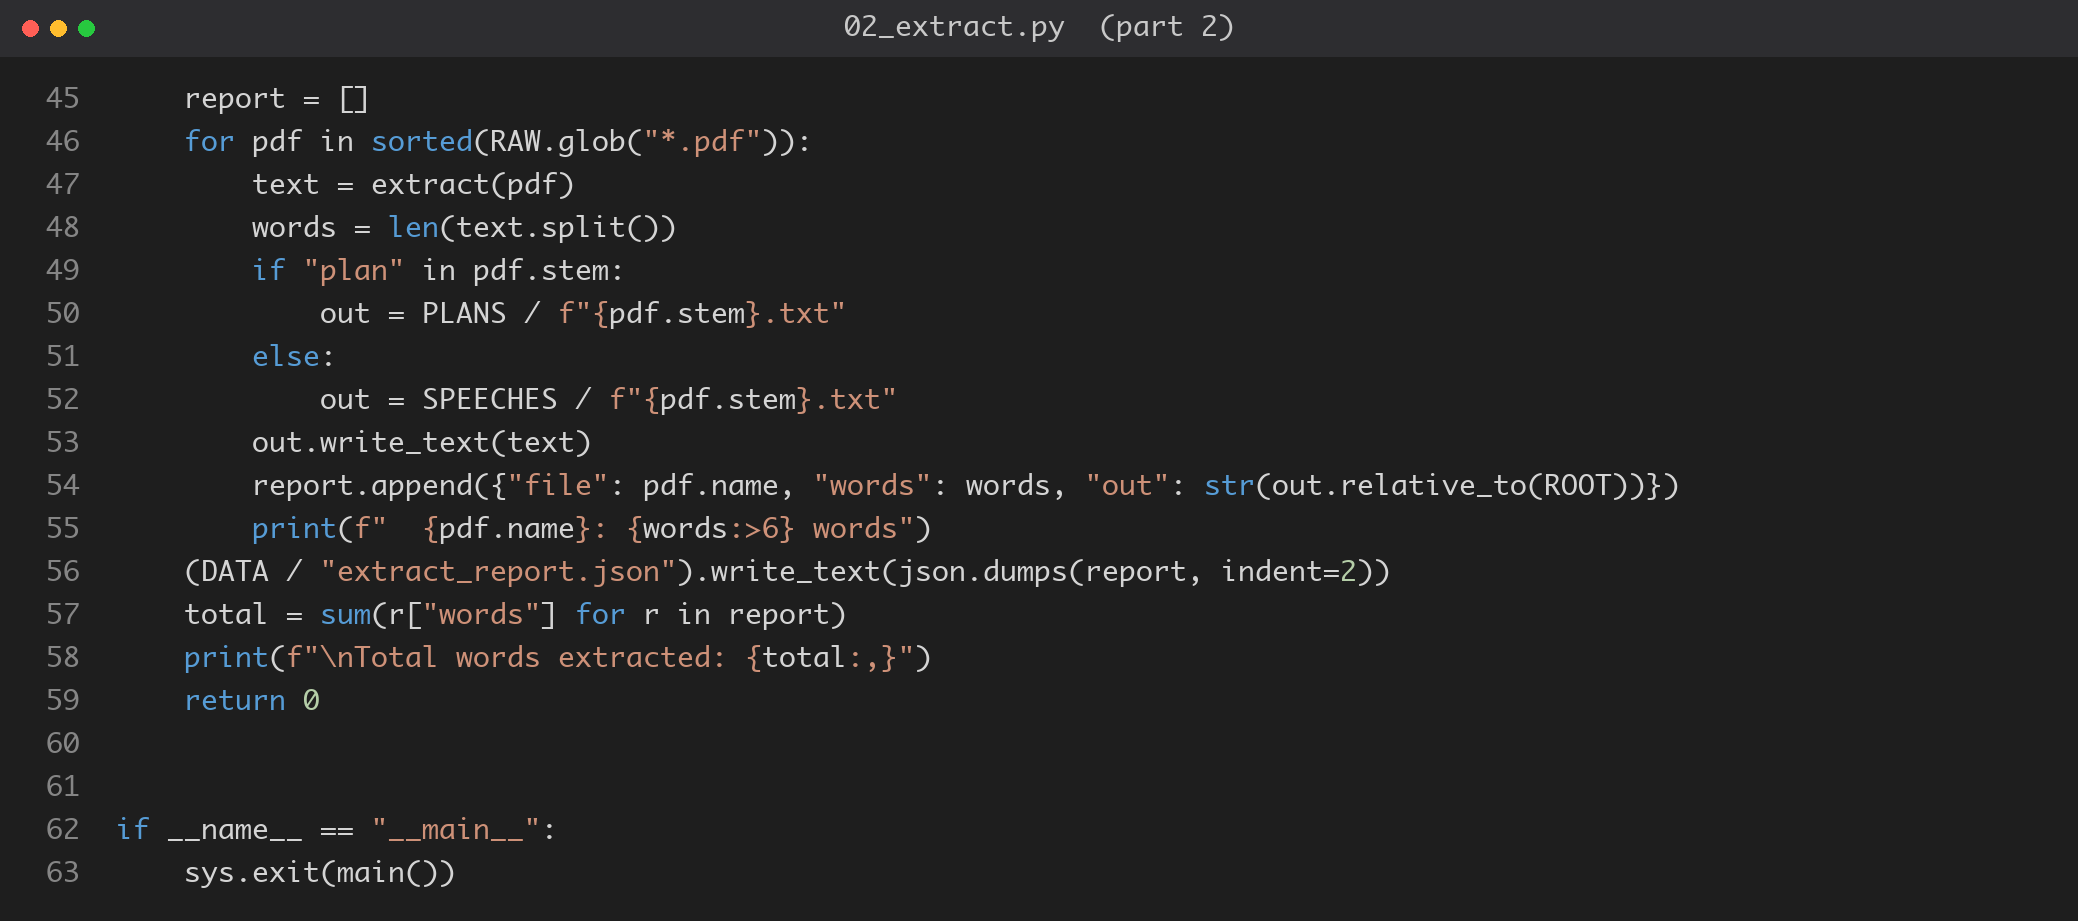
\includegraphics[width=\linewidth]{code_shots/02_extract_py_p2.png}
\subsection{\texttt{03\_analyze.py} --- Preprocessing, LDA, GP models, era classification and figures}
\par\medskip\noindent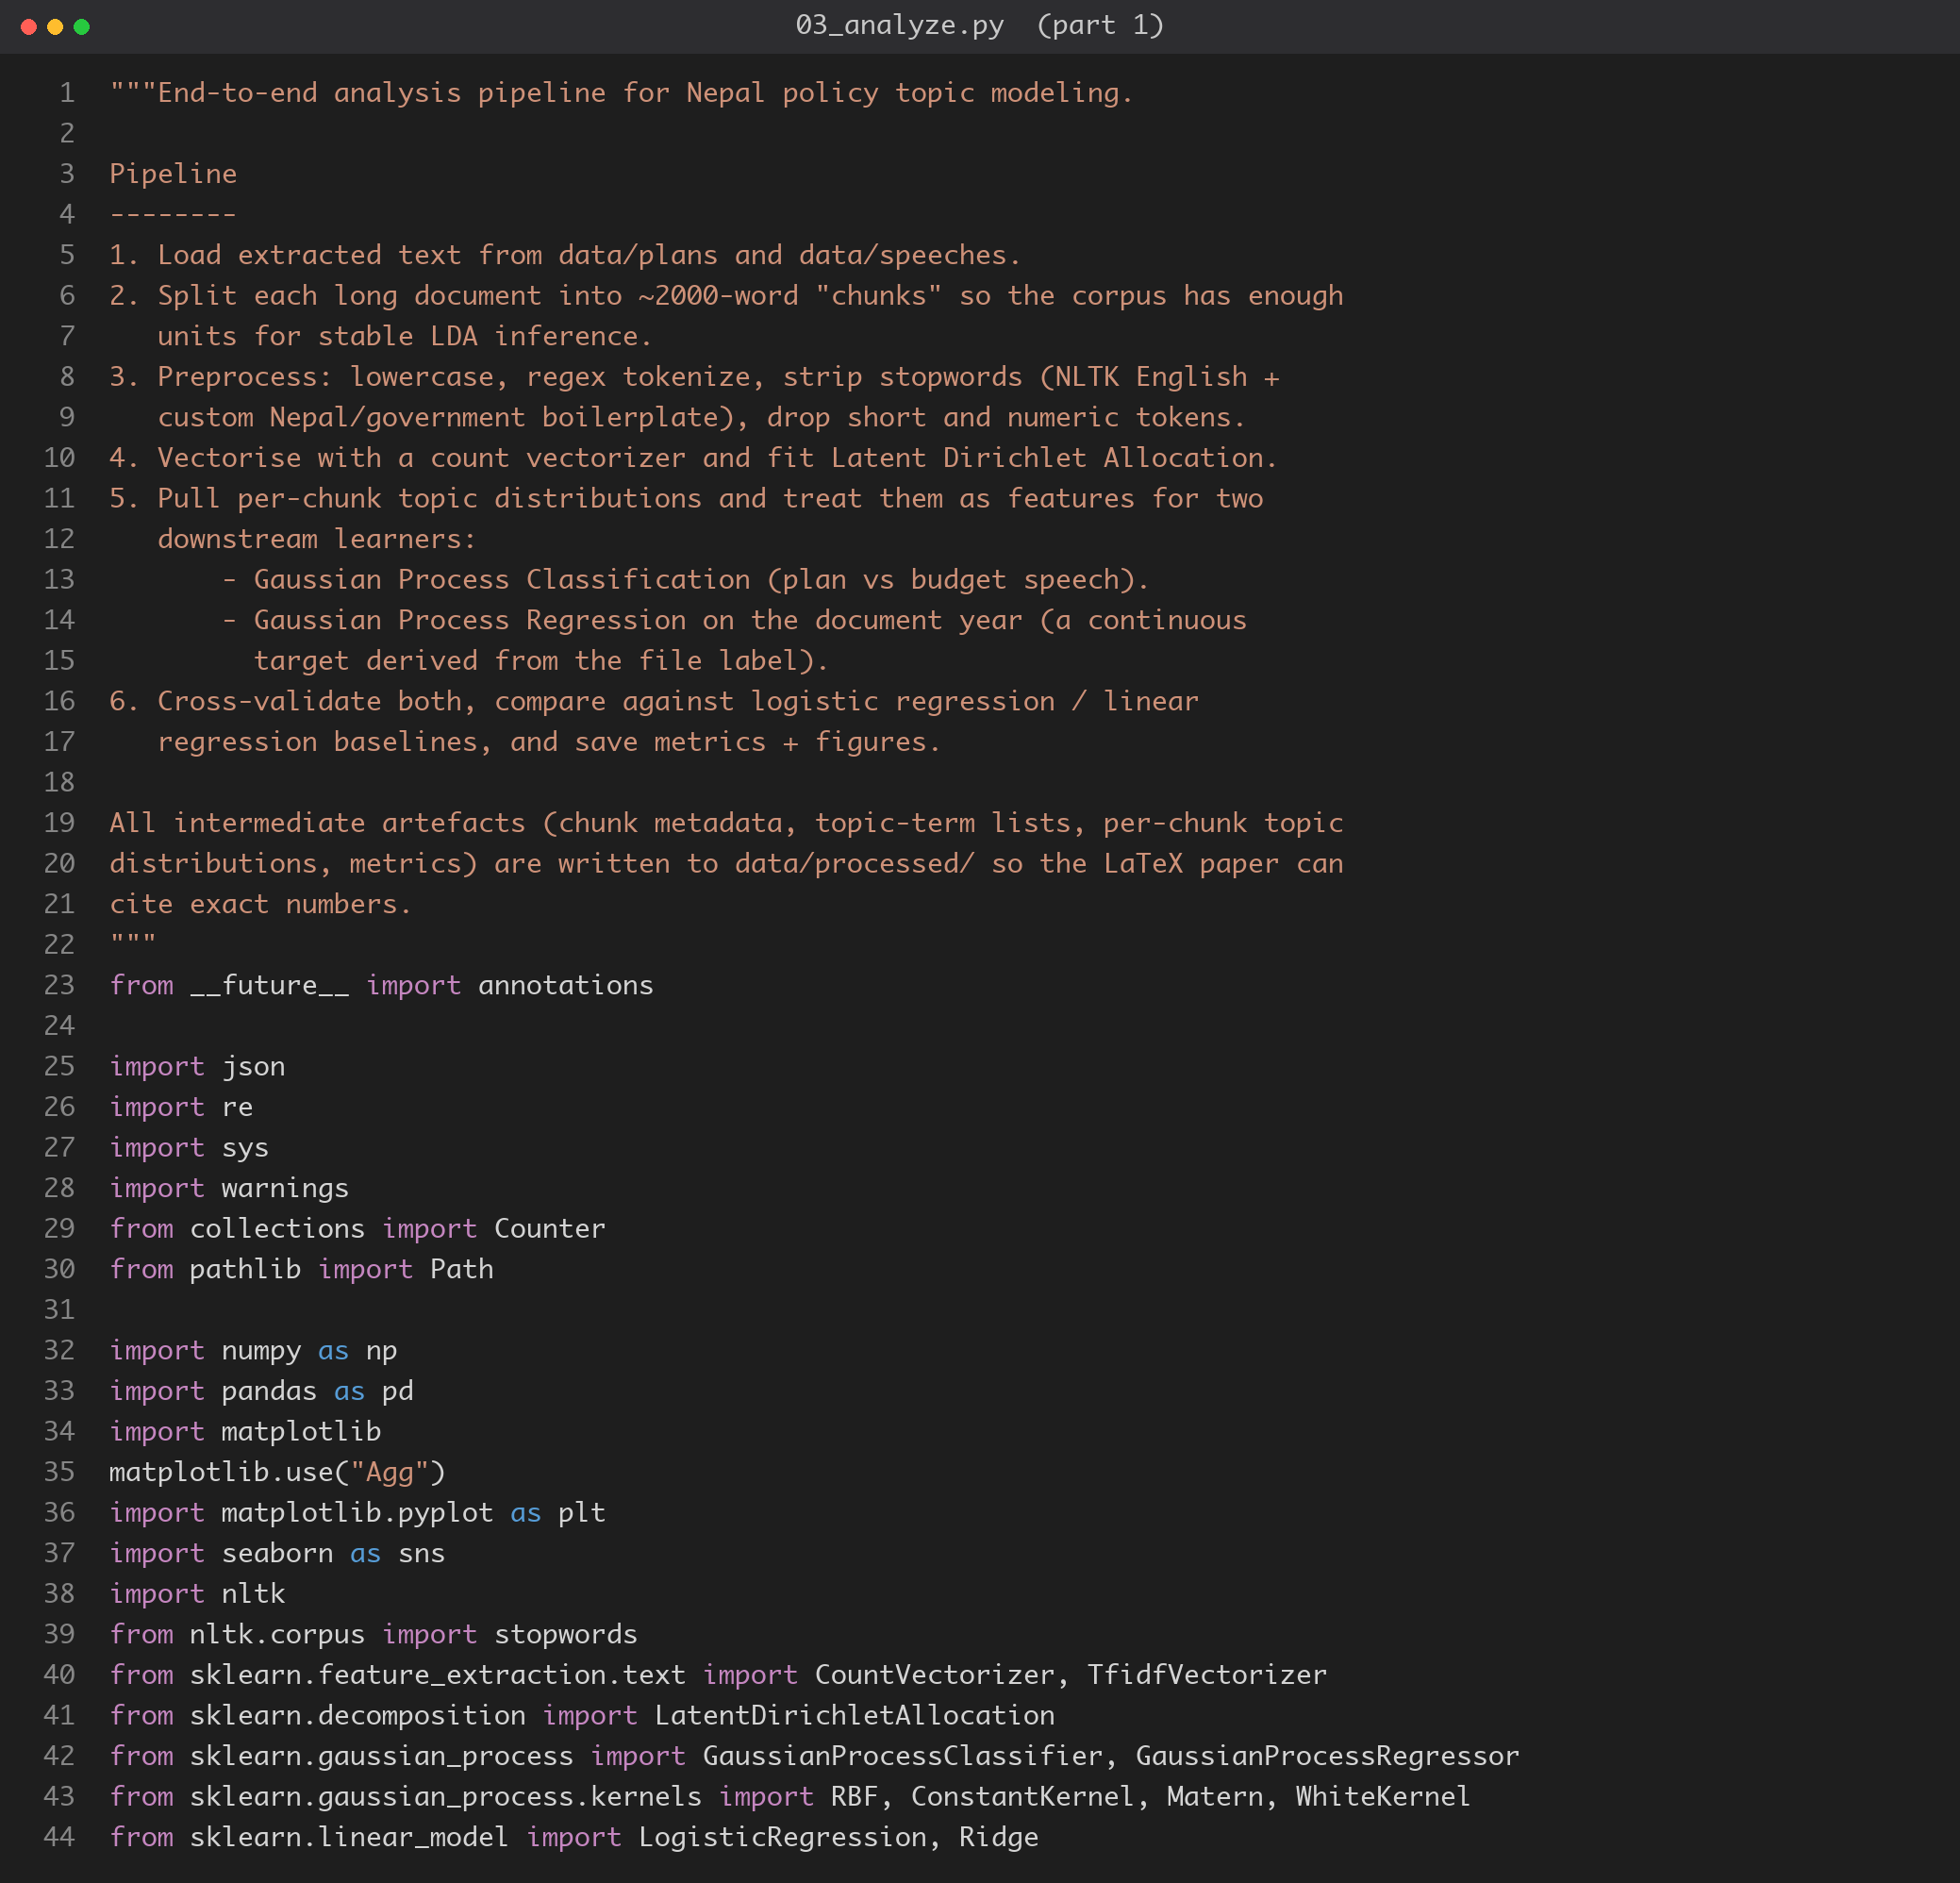
\includegraphics[width=\linewidth]{code_shots/03_analyze_py_p1.png}
\par\medskip\noindent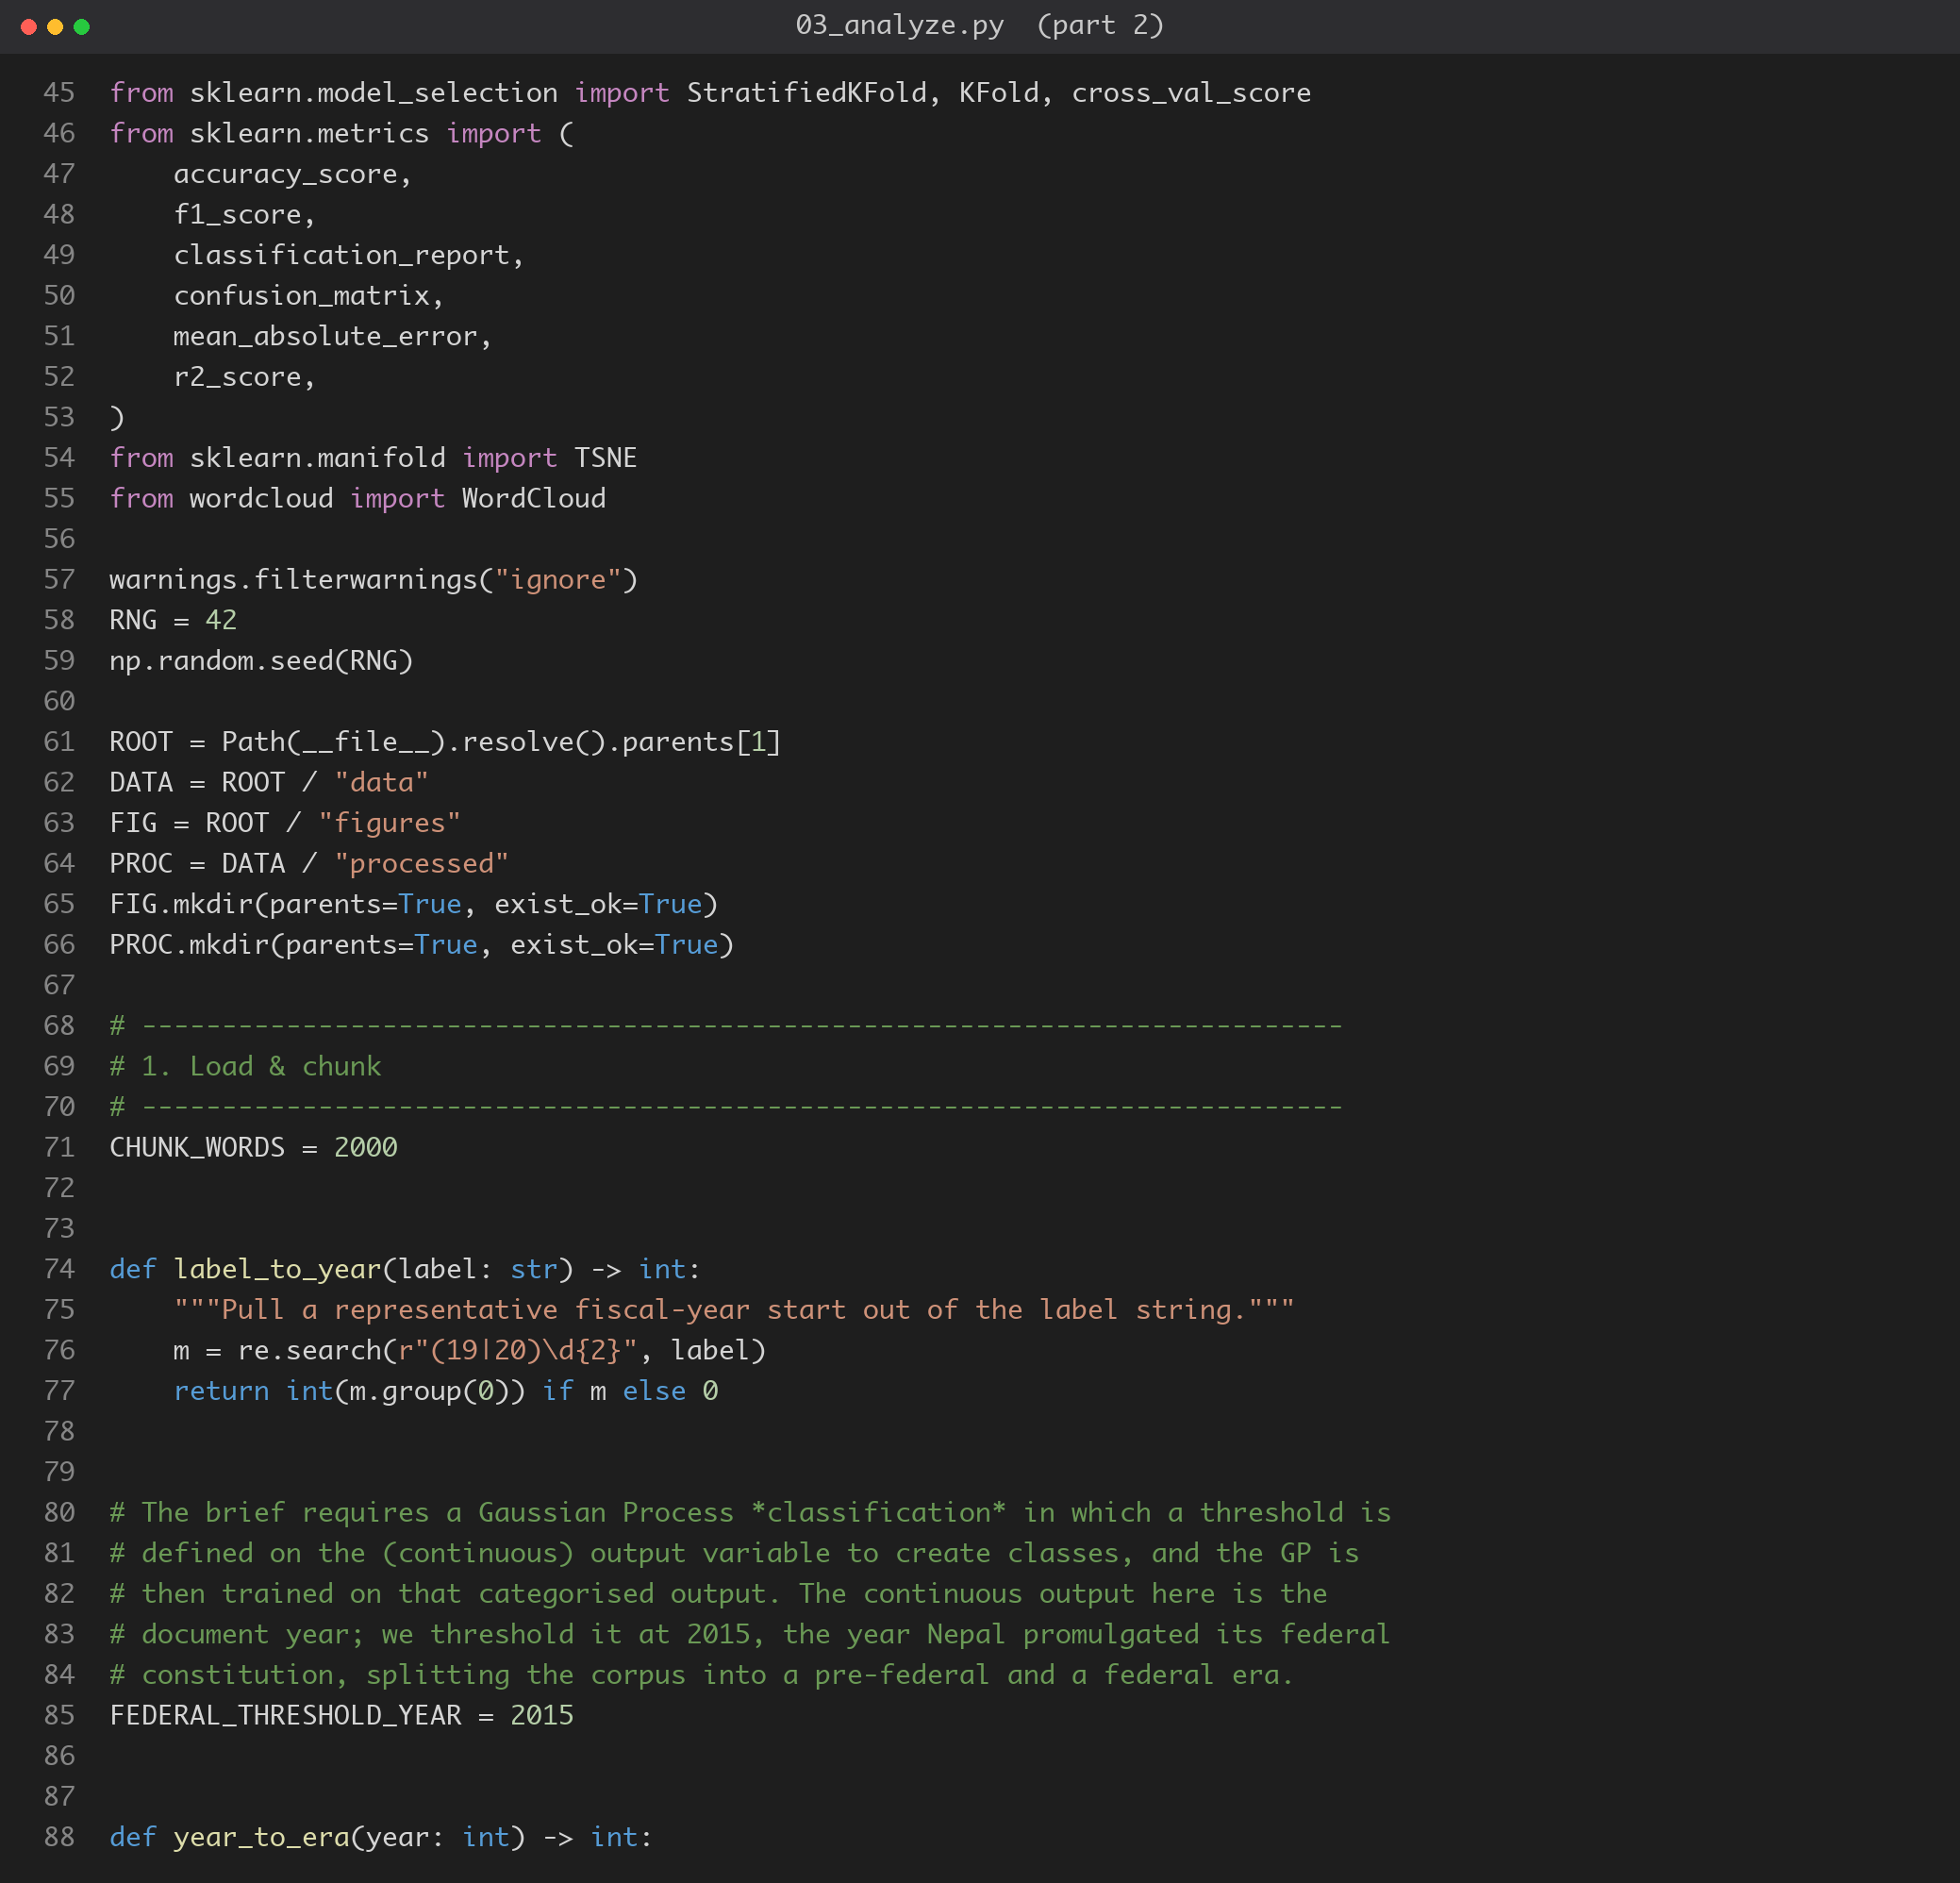
\includegraphics[width=\linewidth]{code_shots/03_analyze_py_p2.png}
\par\medskip\noindent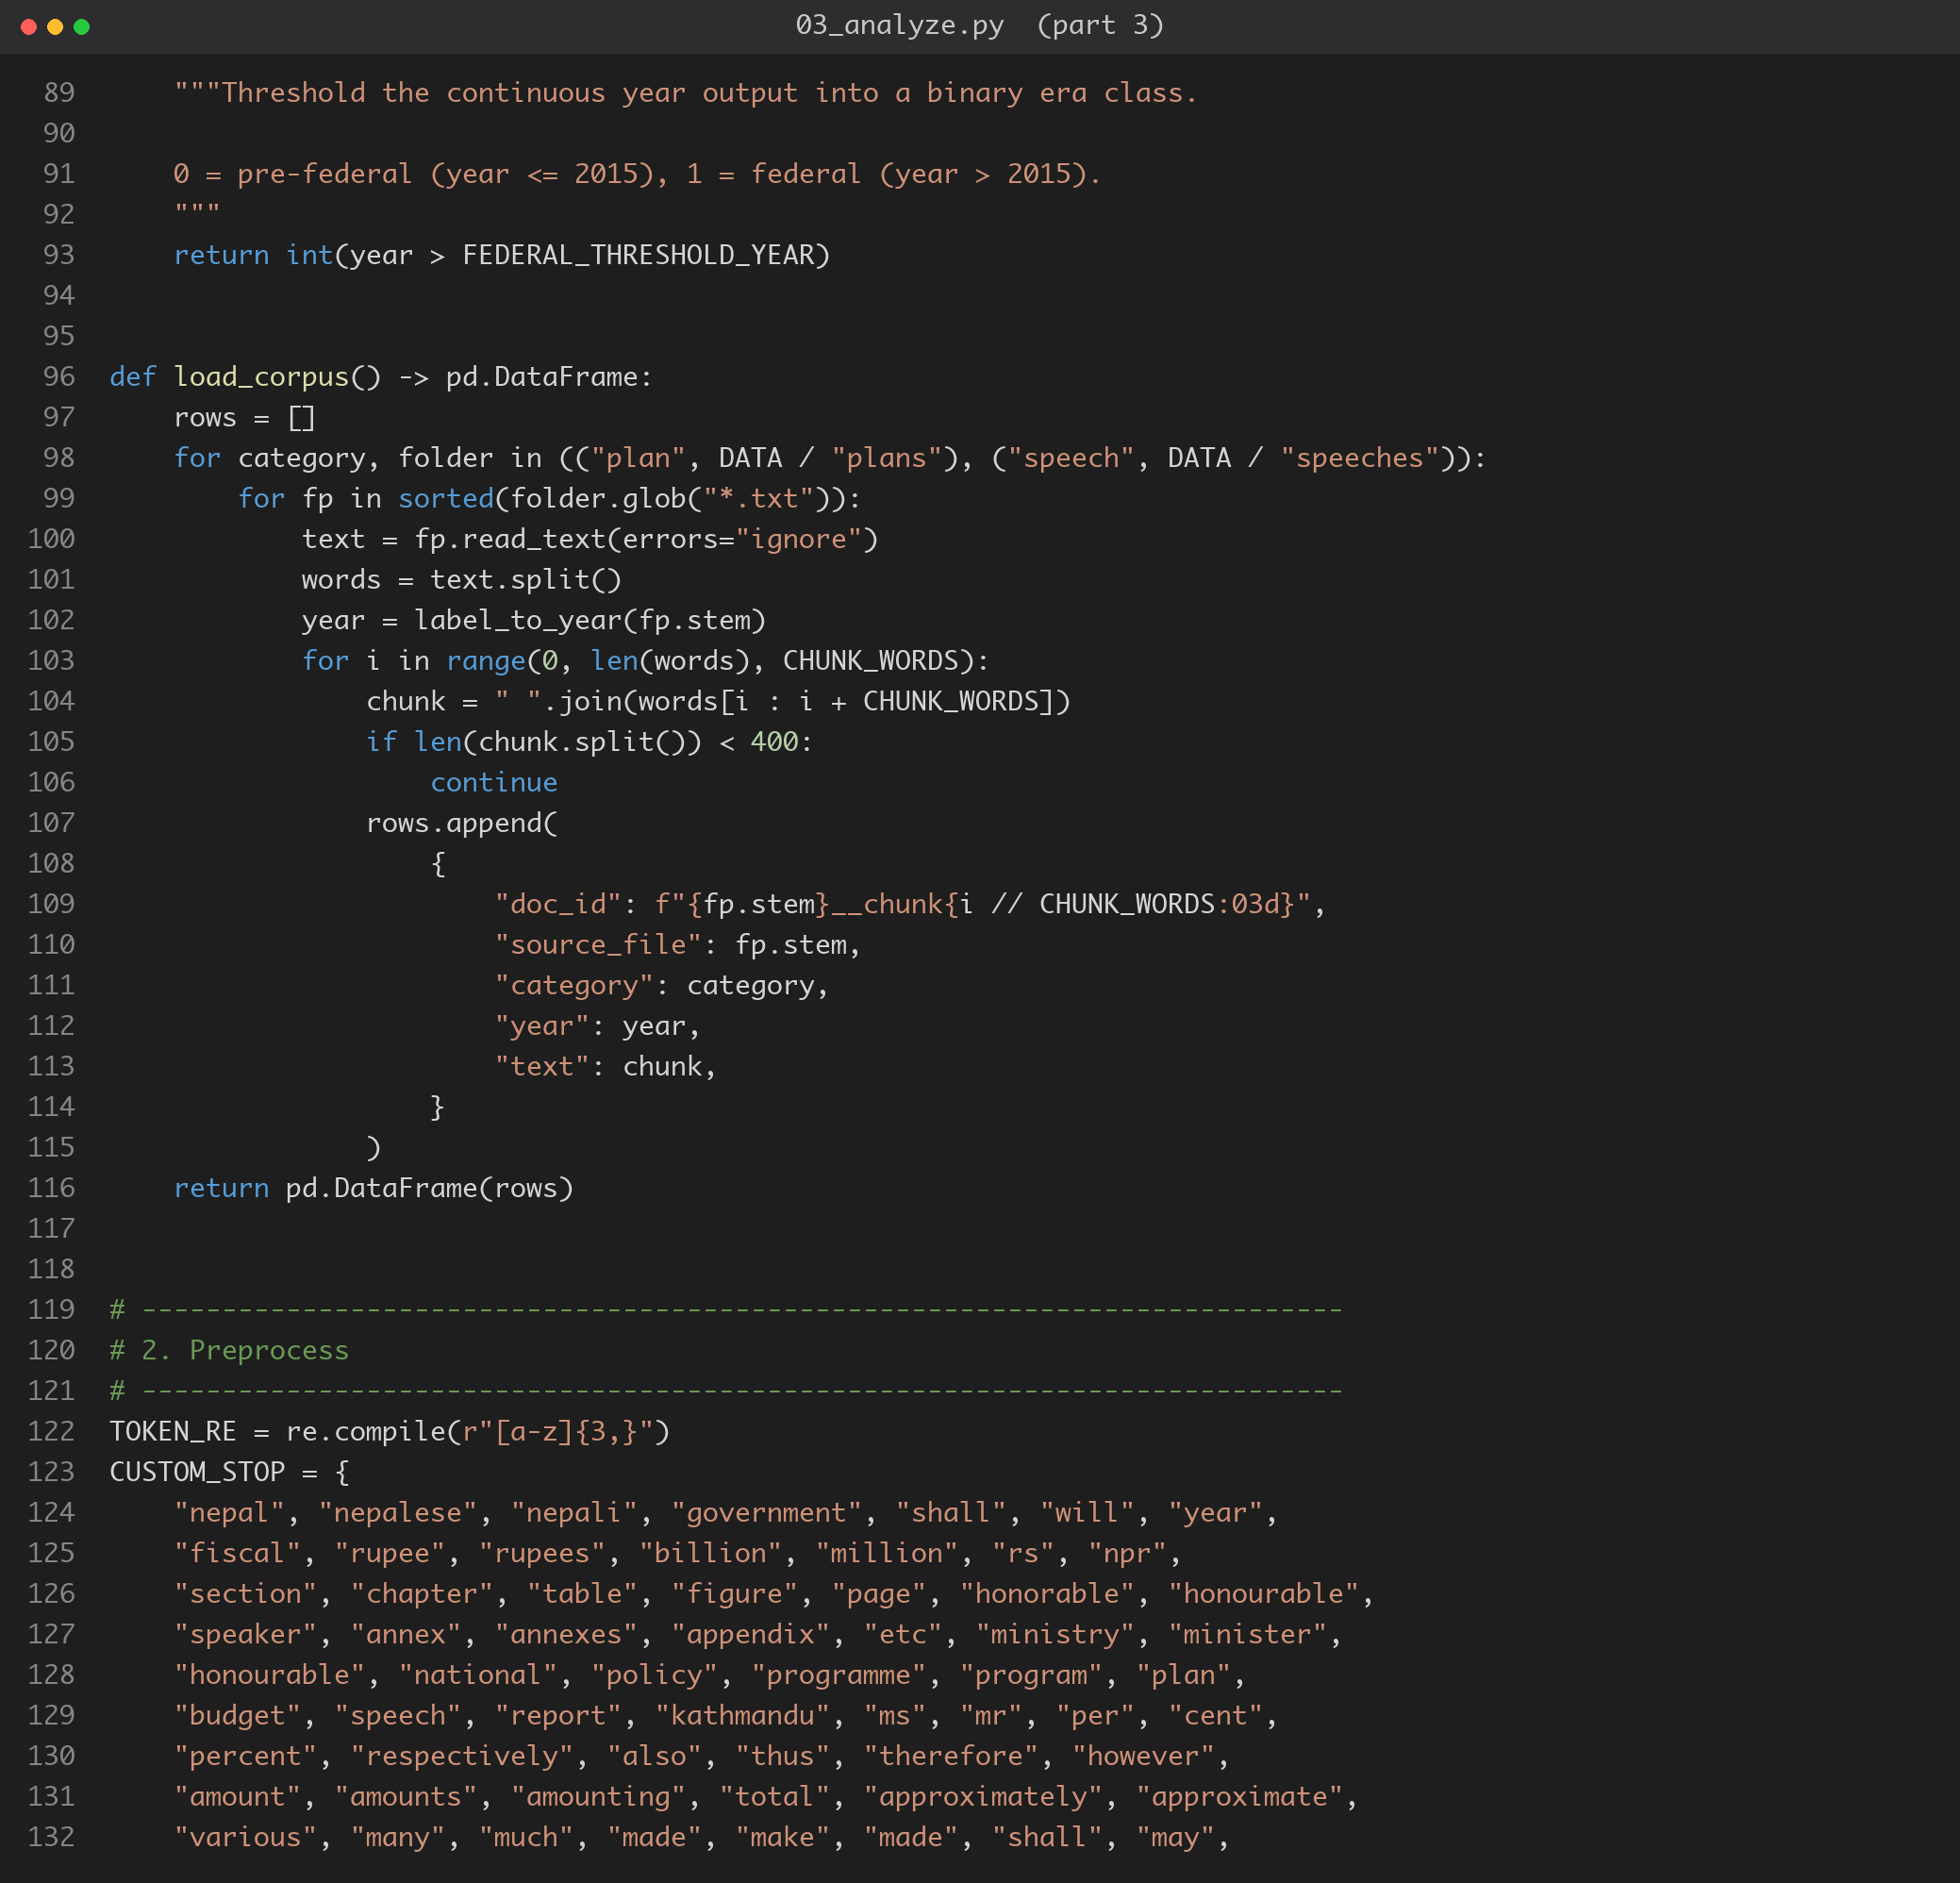
\includegraphics[width=\linewidth]{code_shots/03_analyze_py_p3.png}
\par\medskip\noindent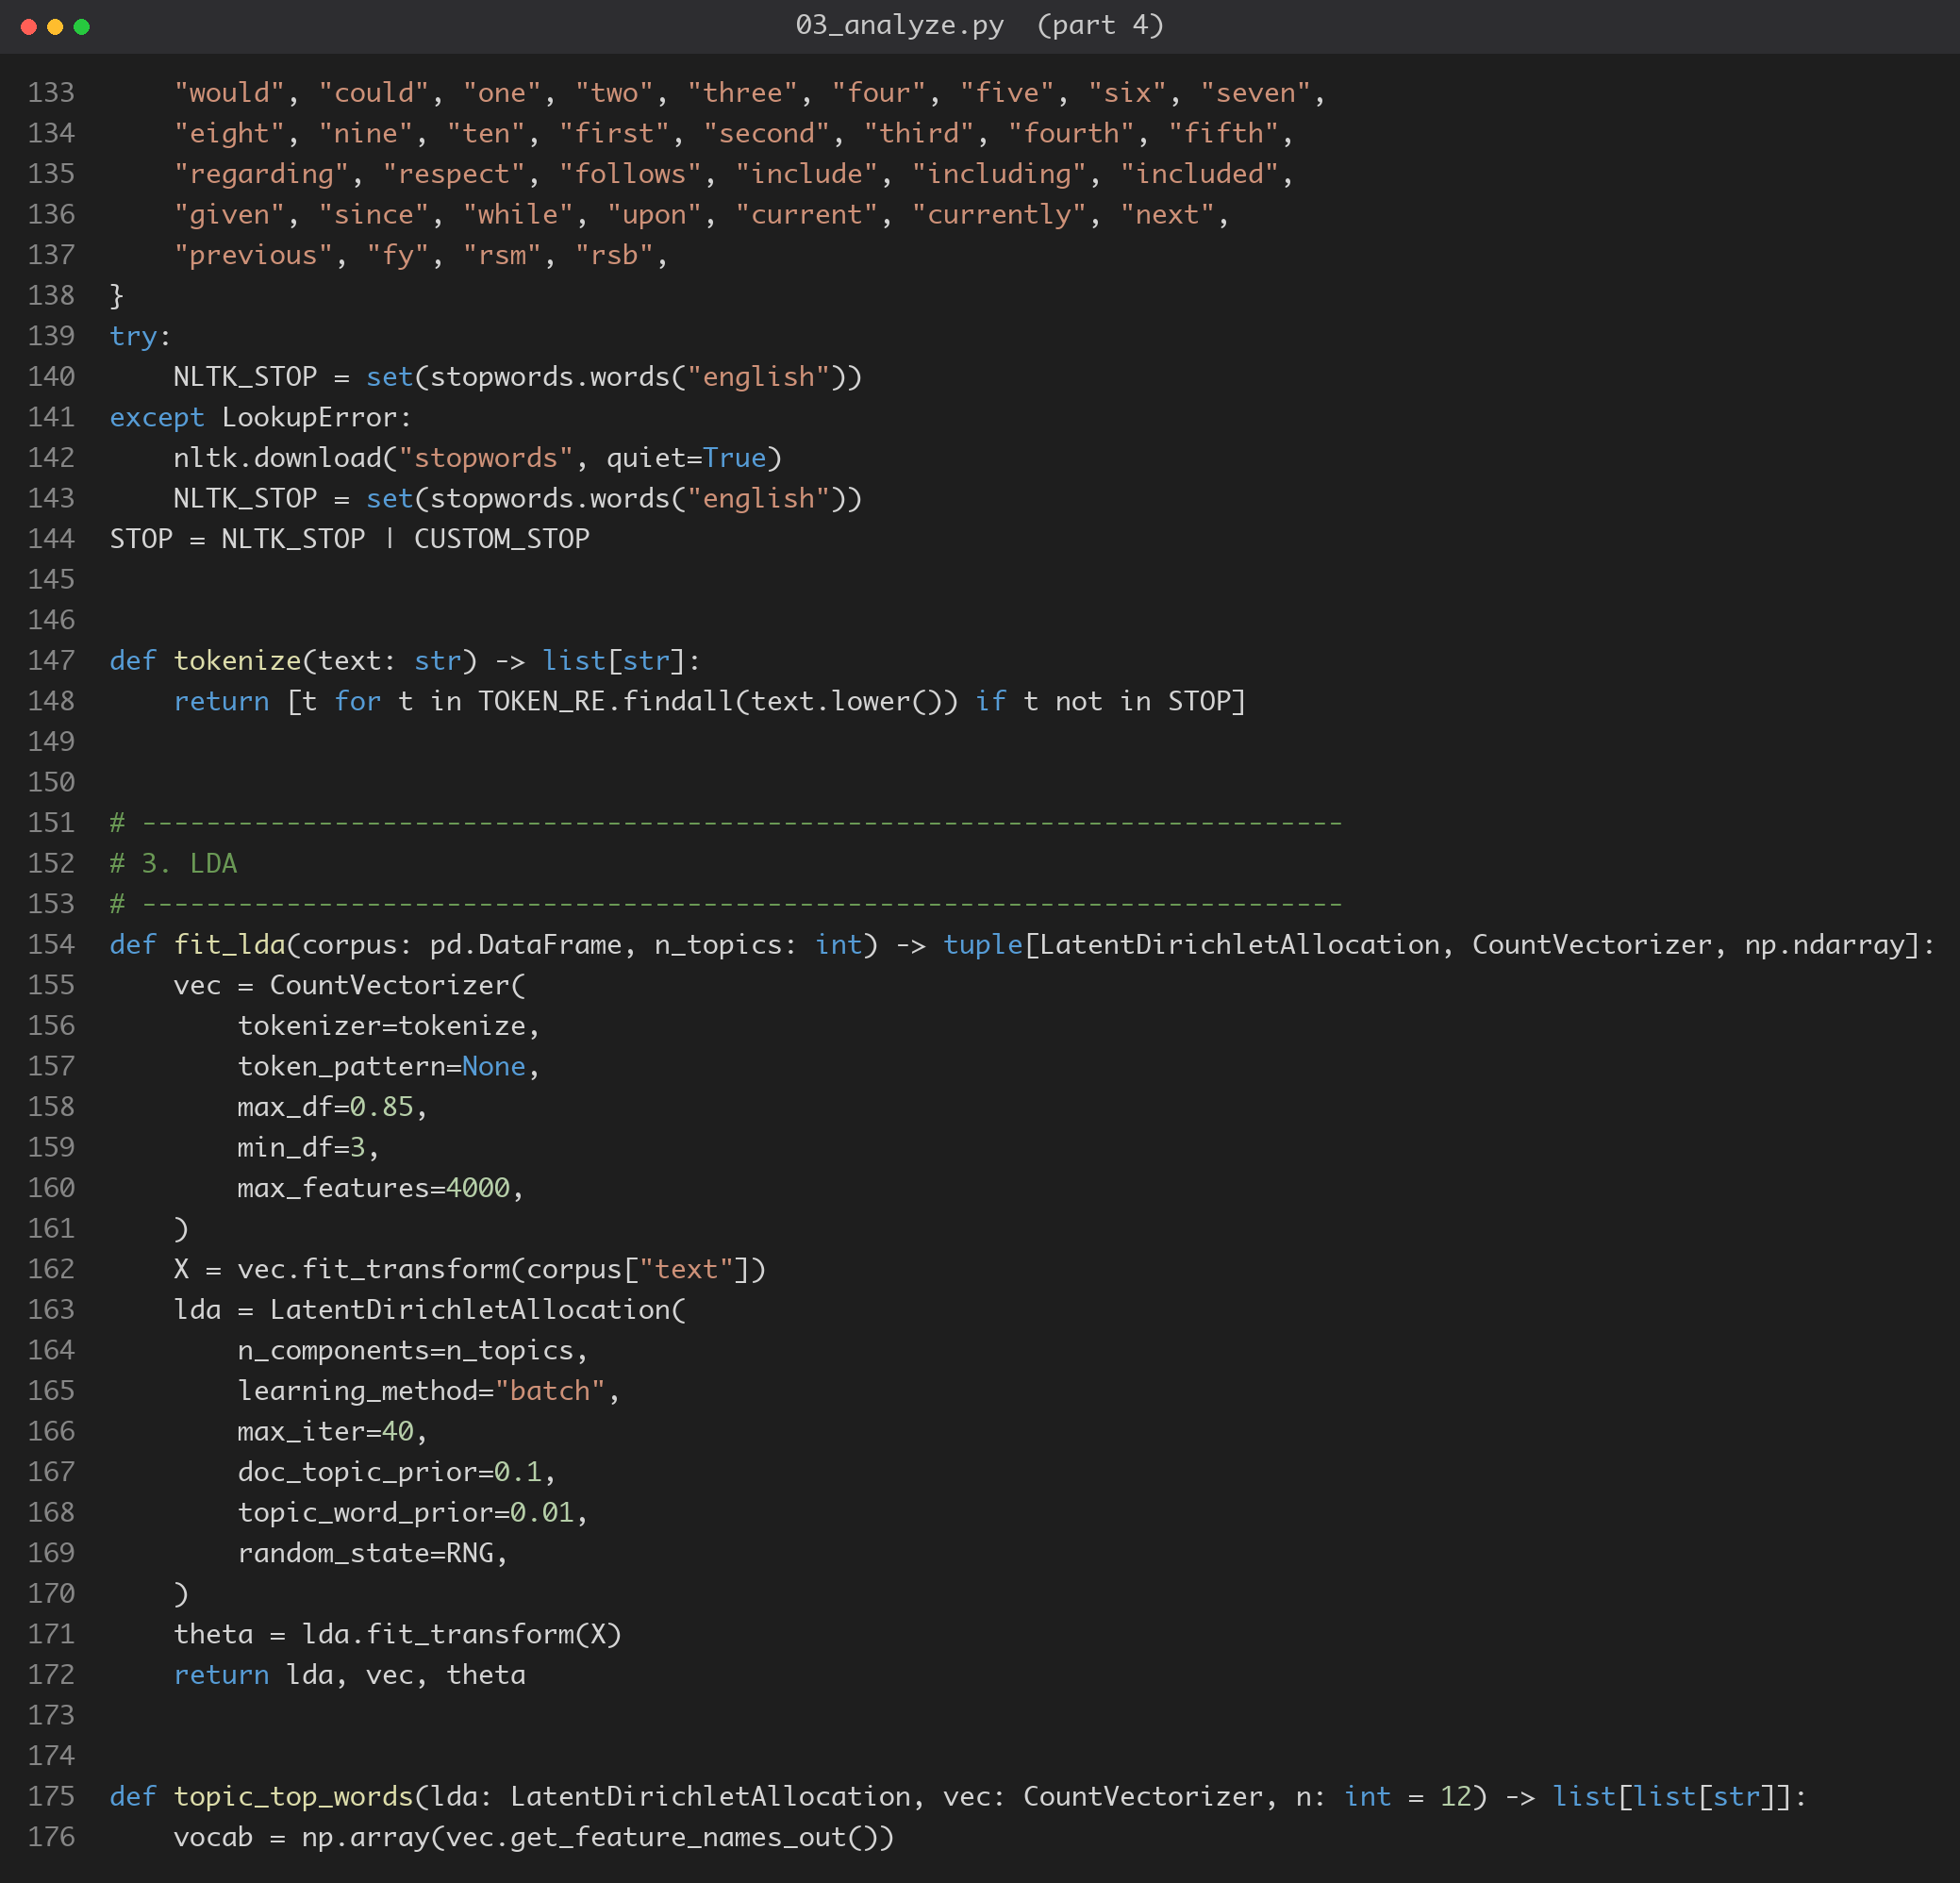
\includegraphics[width=\linewidth]{code_shots/03_analyze_py_p4.png}
\par\medskip\noindent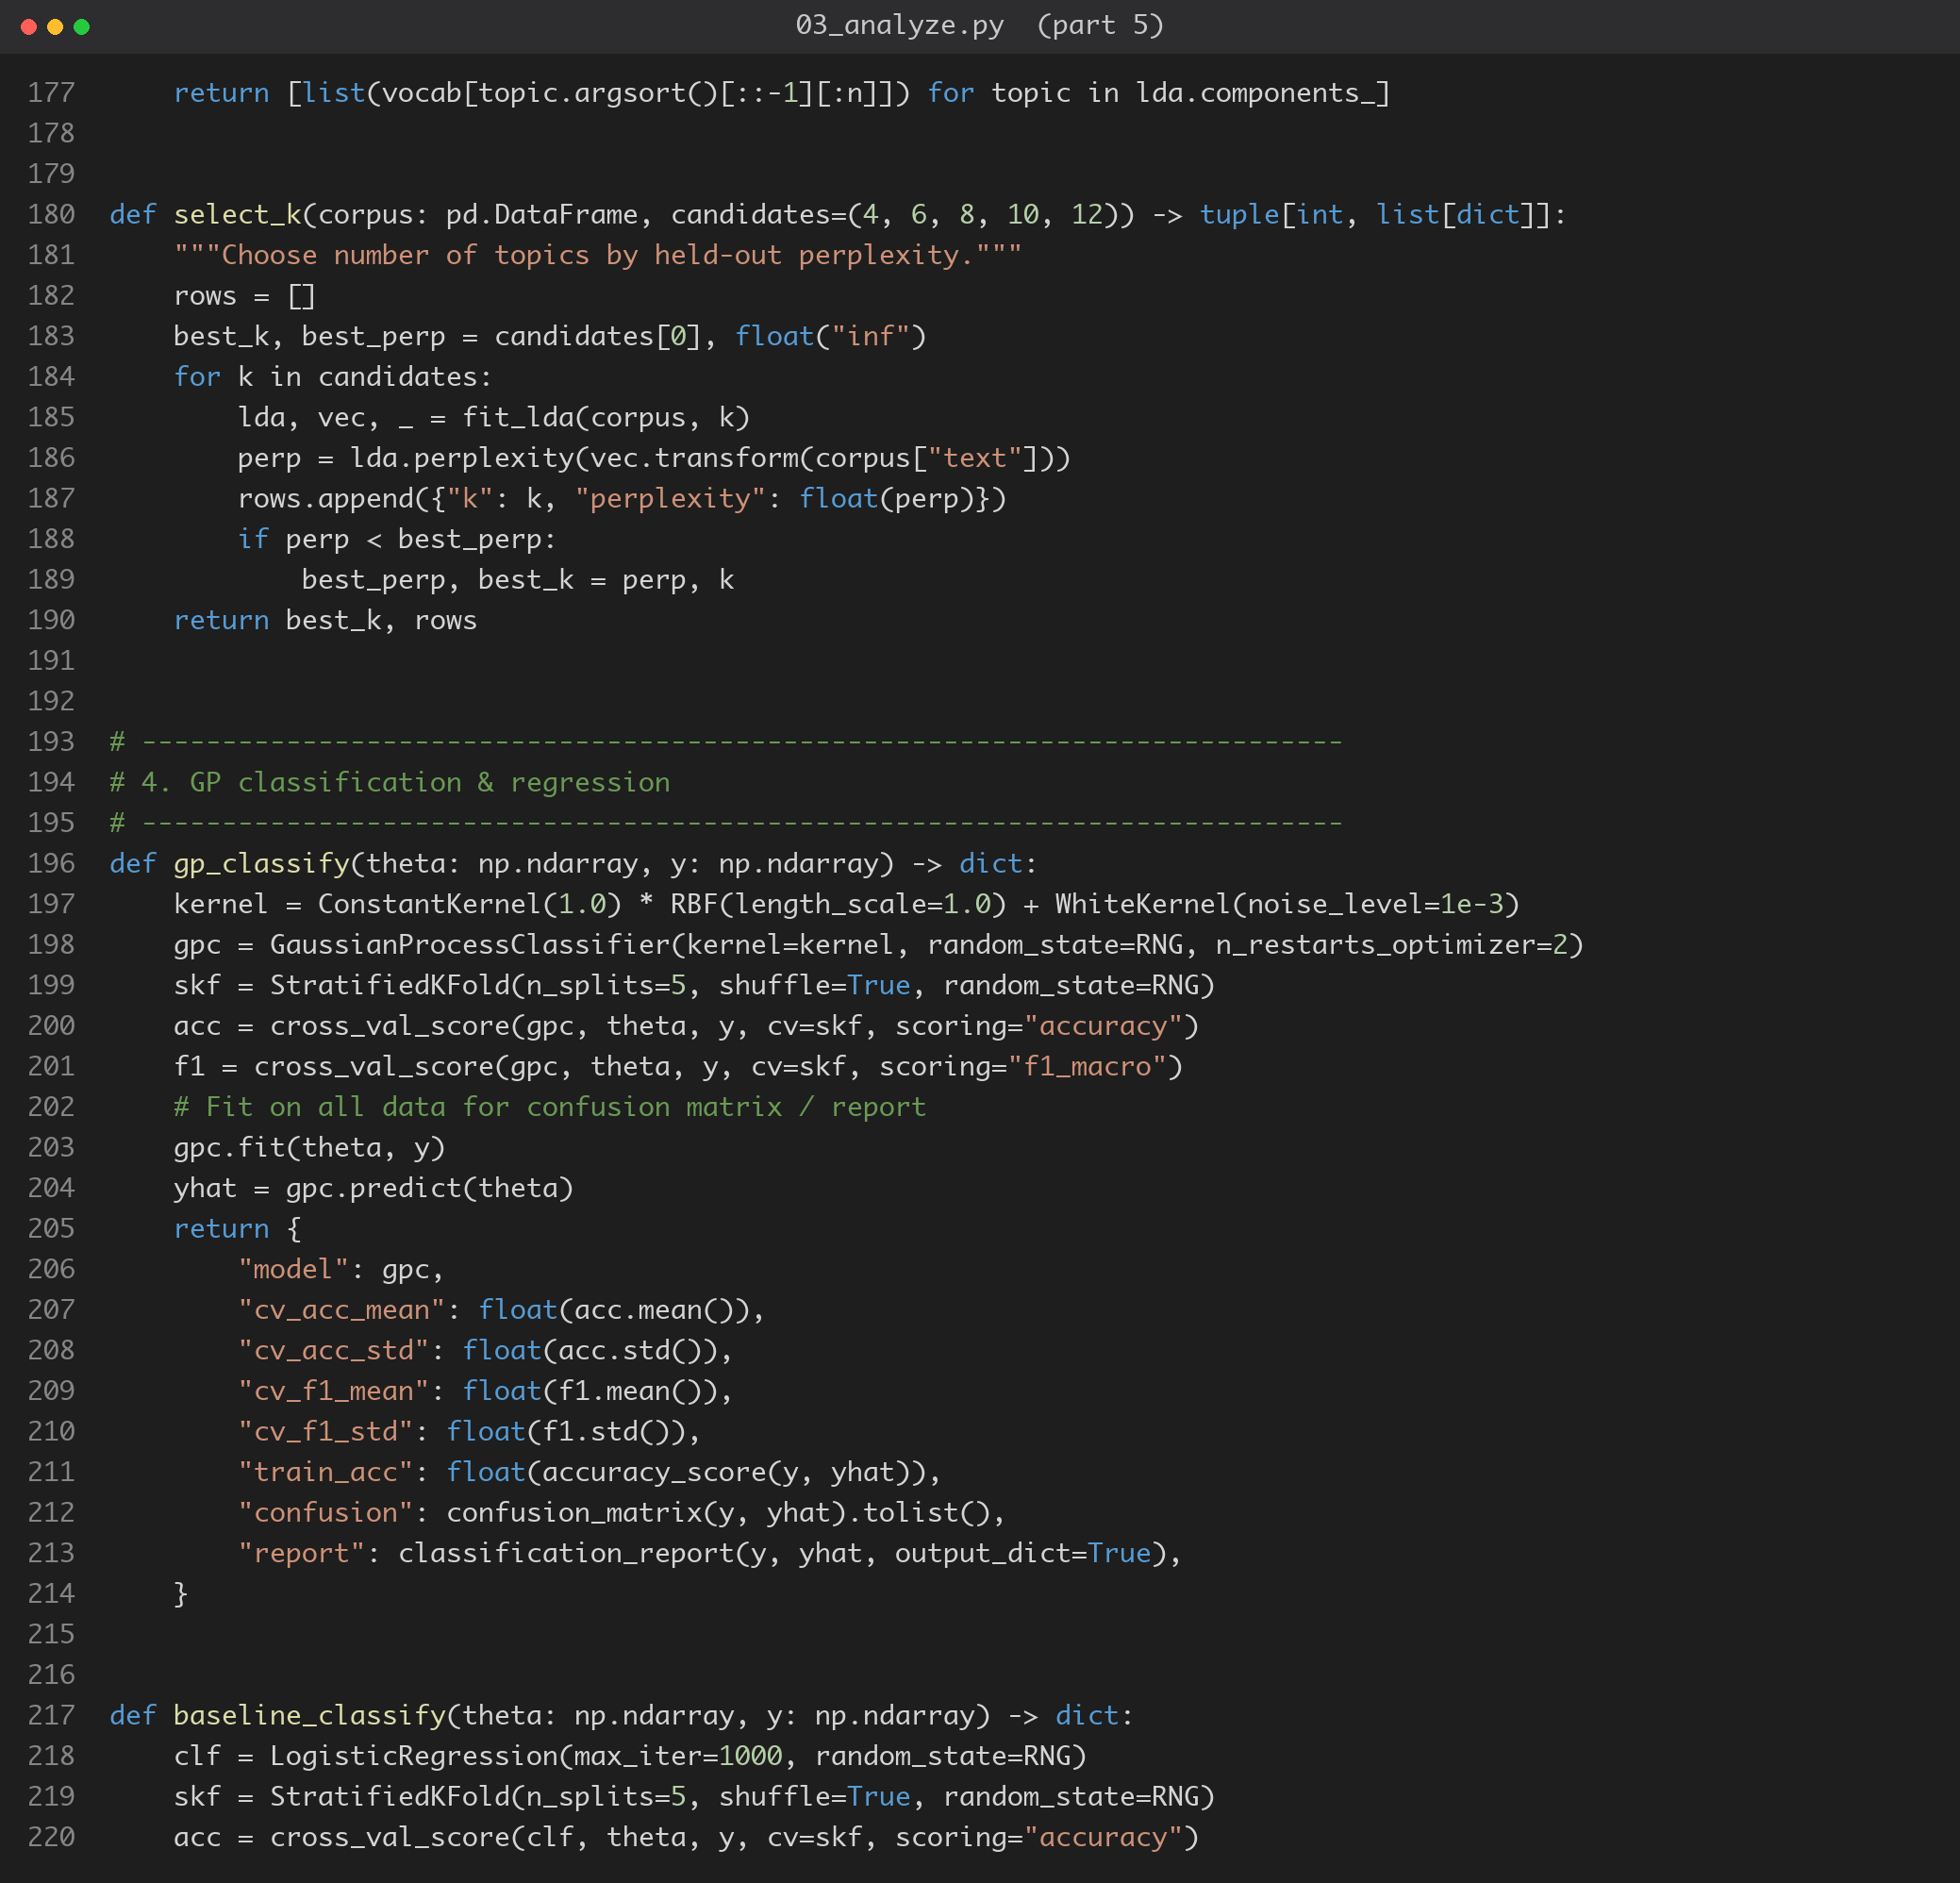
\includegraphics[width=\linewidth]{code_shots/03_analyze_py_p5.png}
\par\medskip\noindent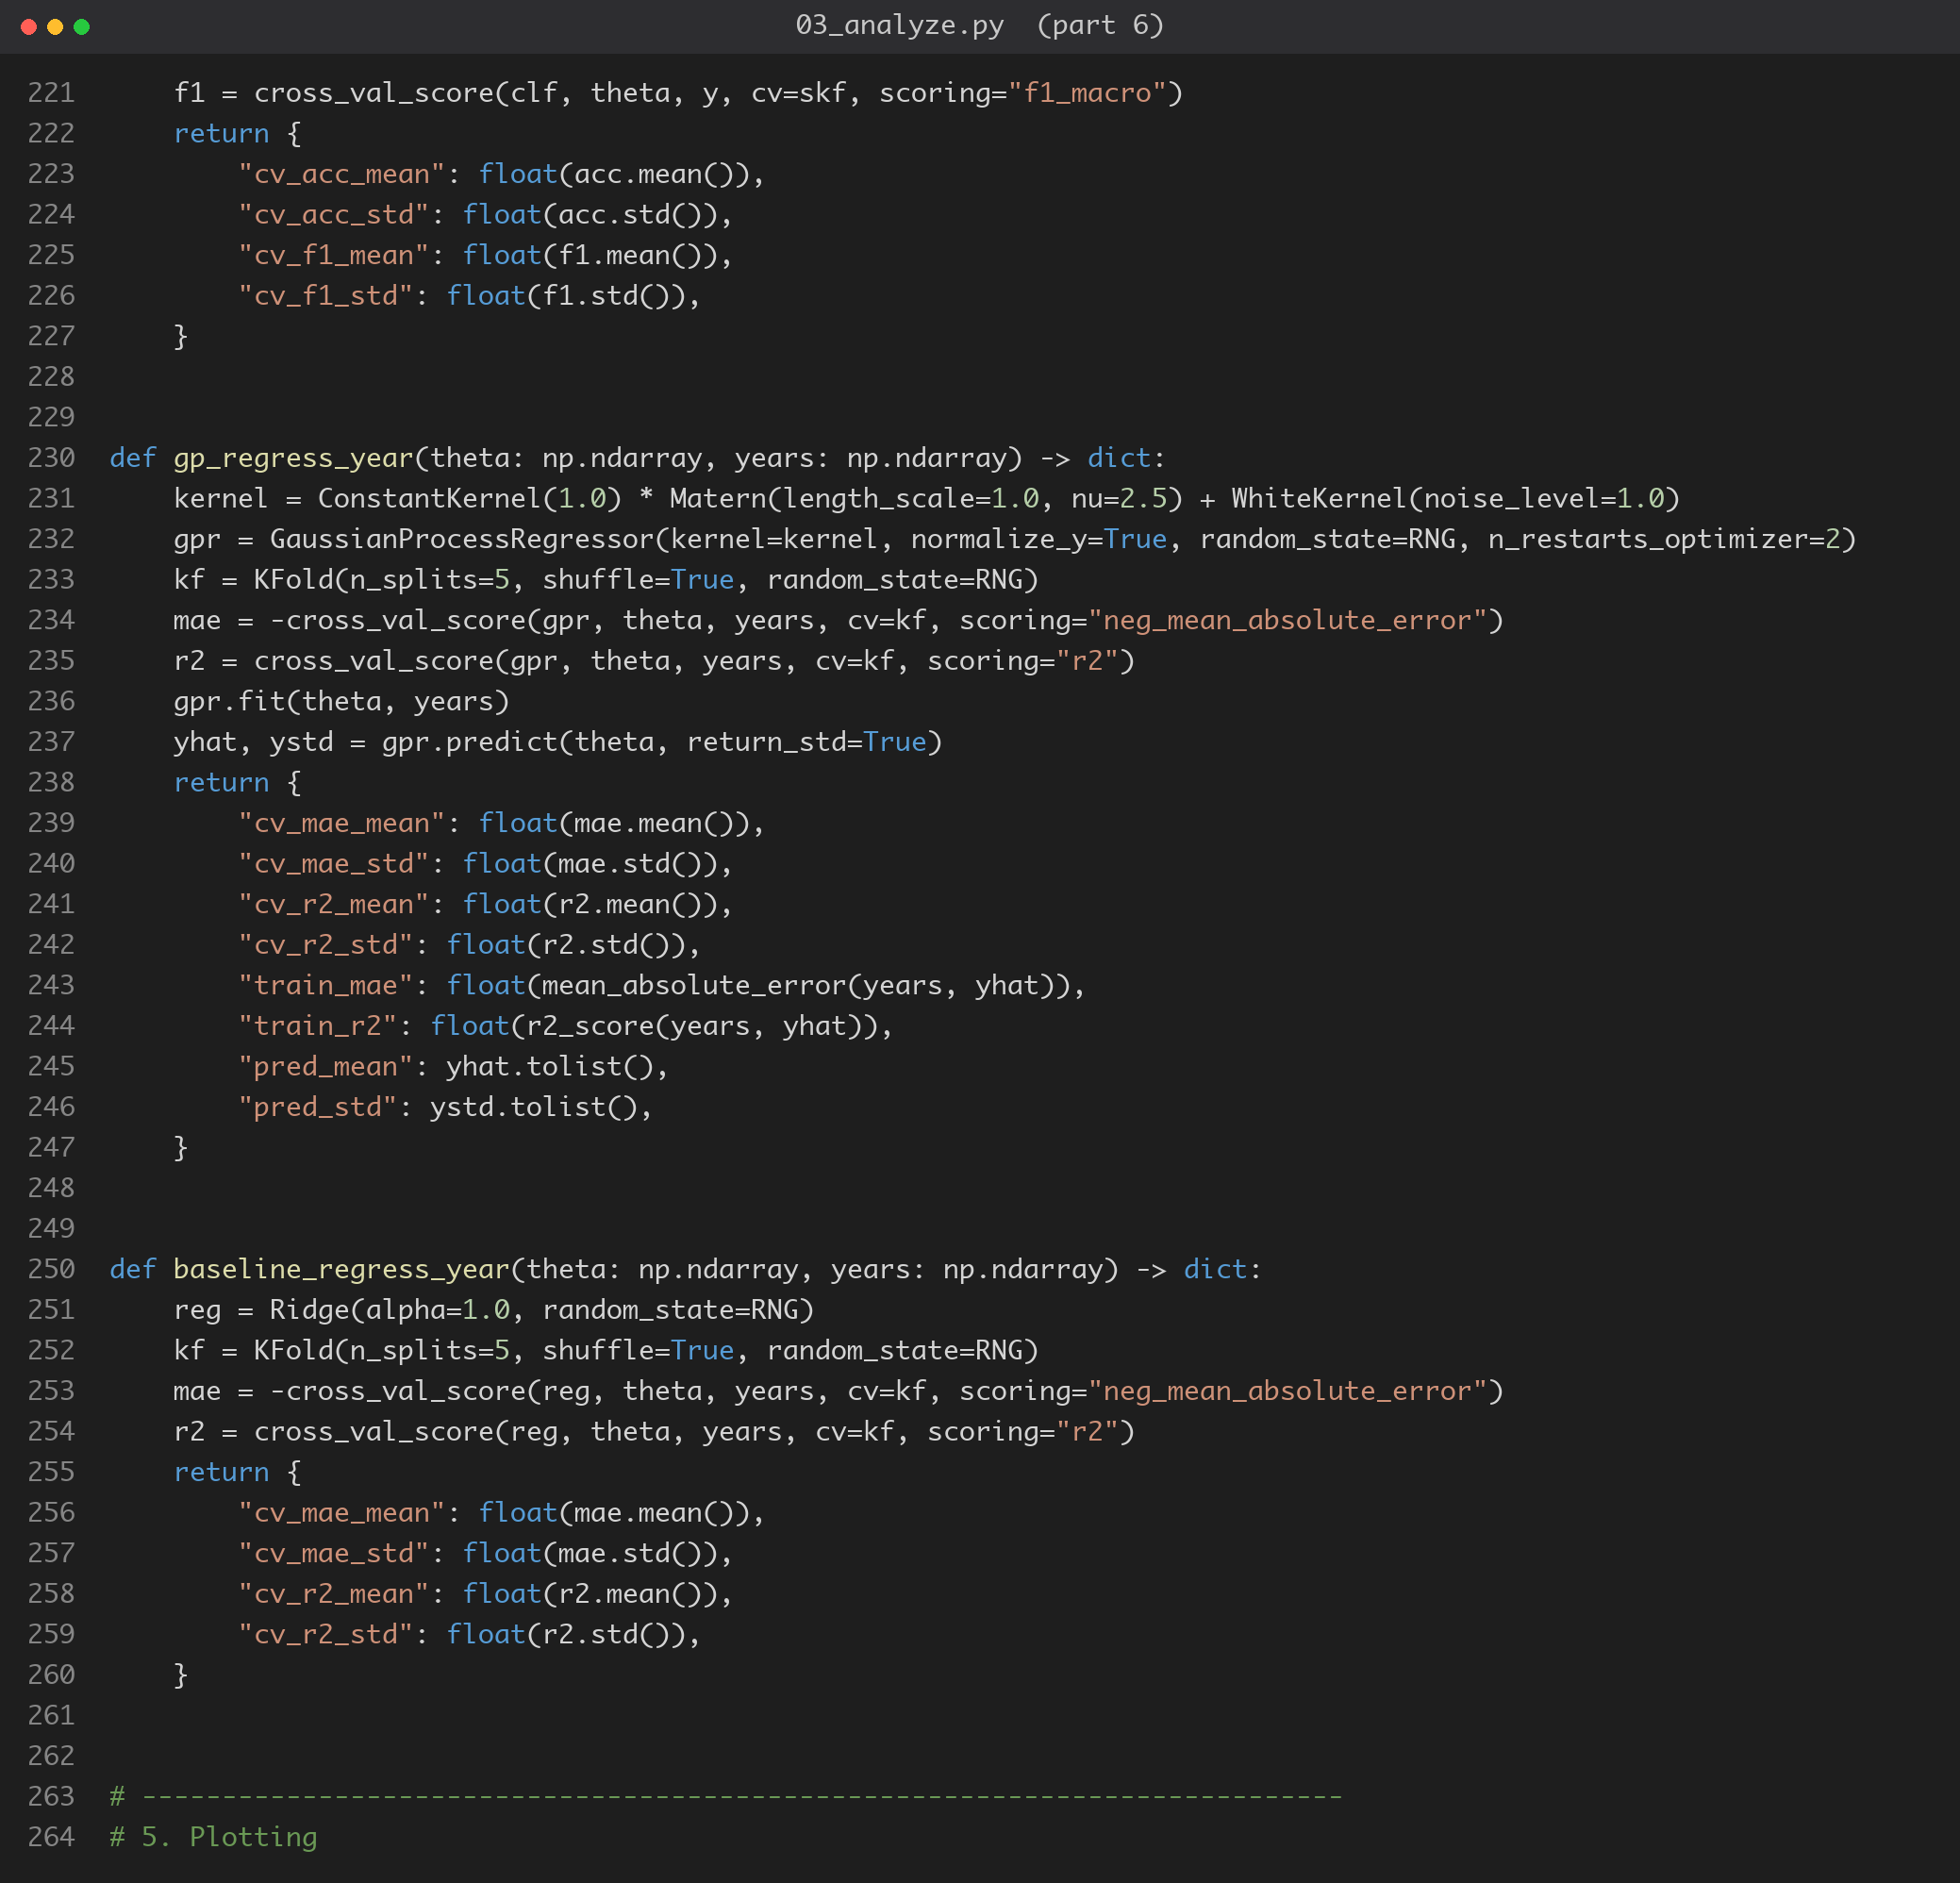
\includegraphics[width=\linewidth]{code_shots/03_analyze_py_p6.png}
\par\medskip\noindent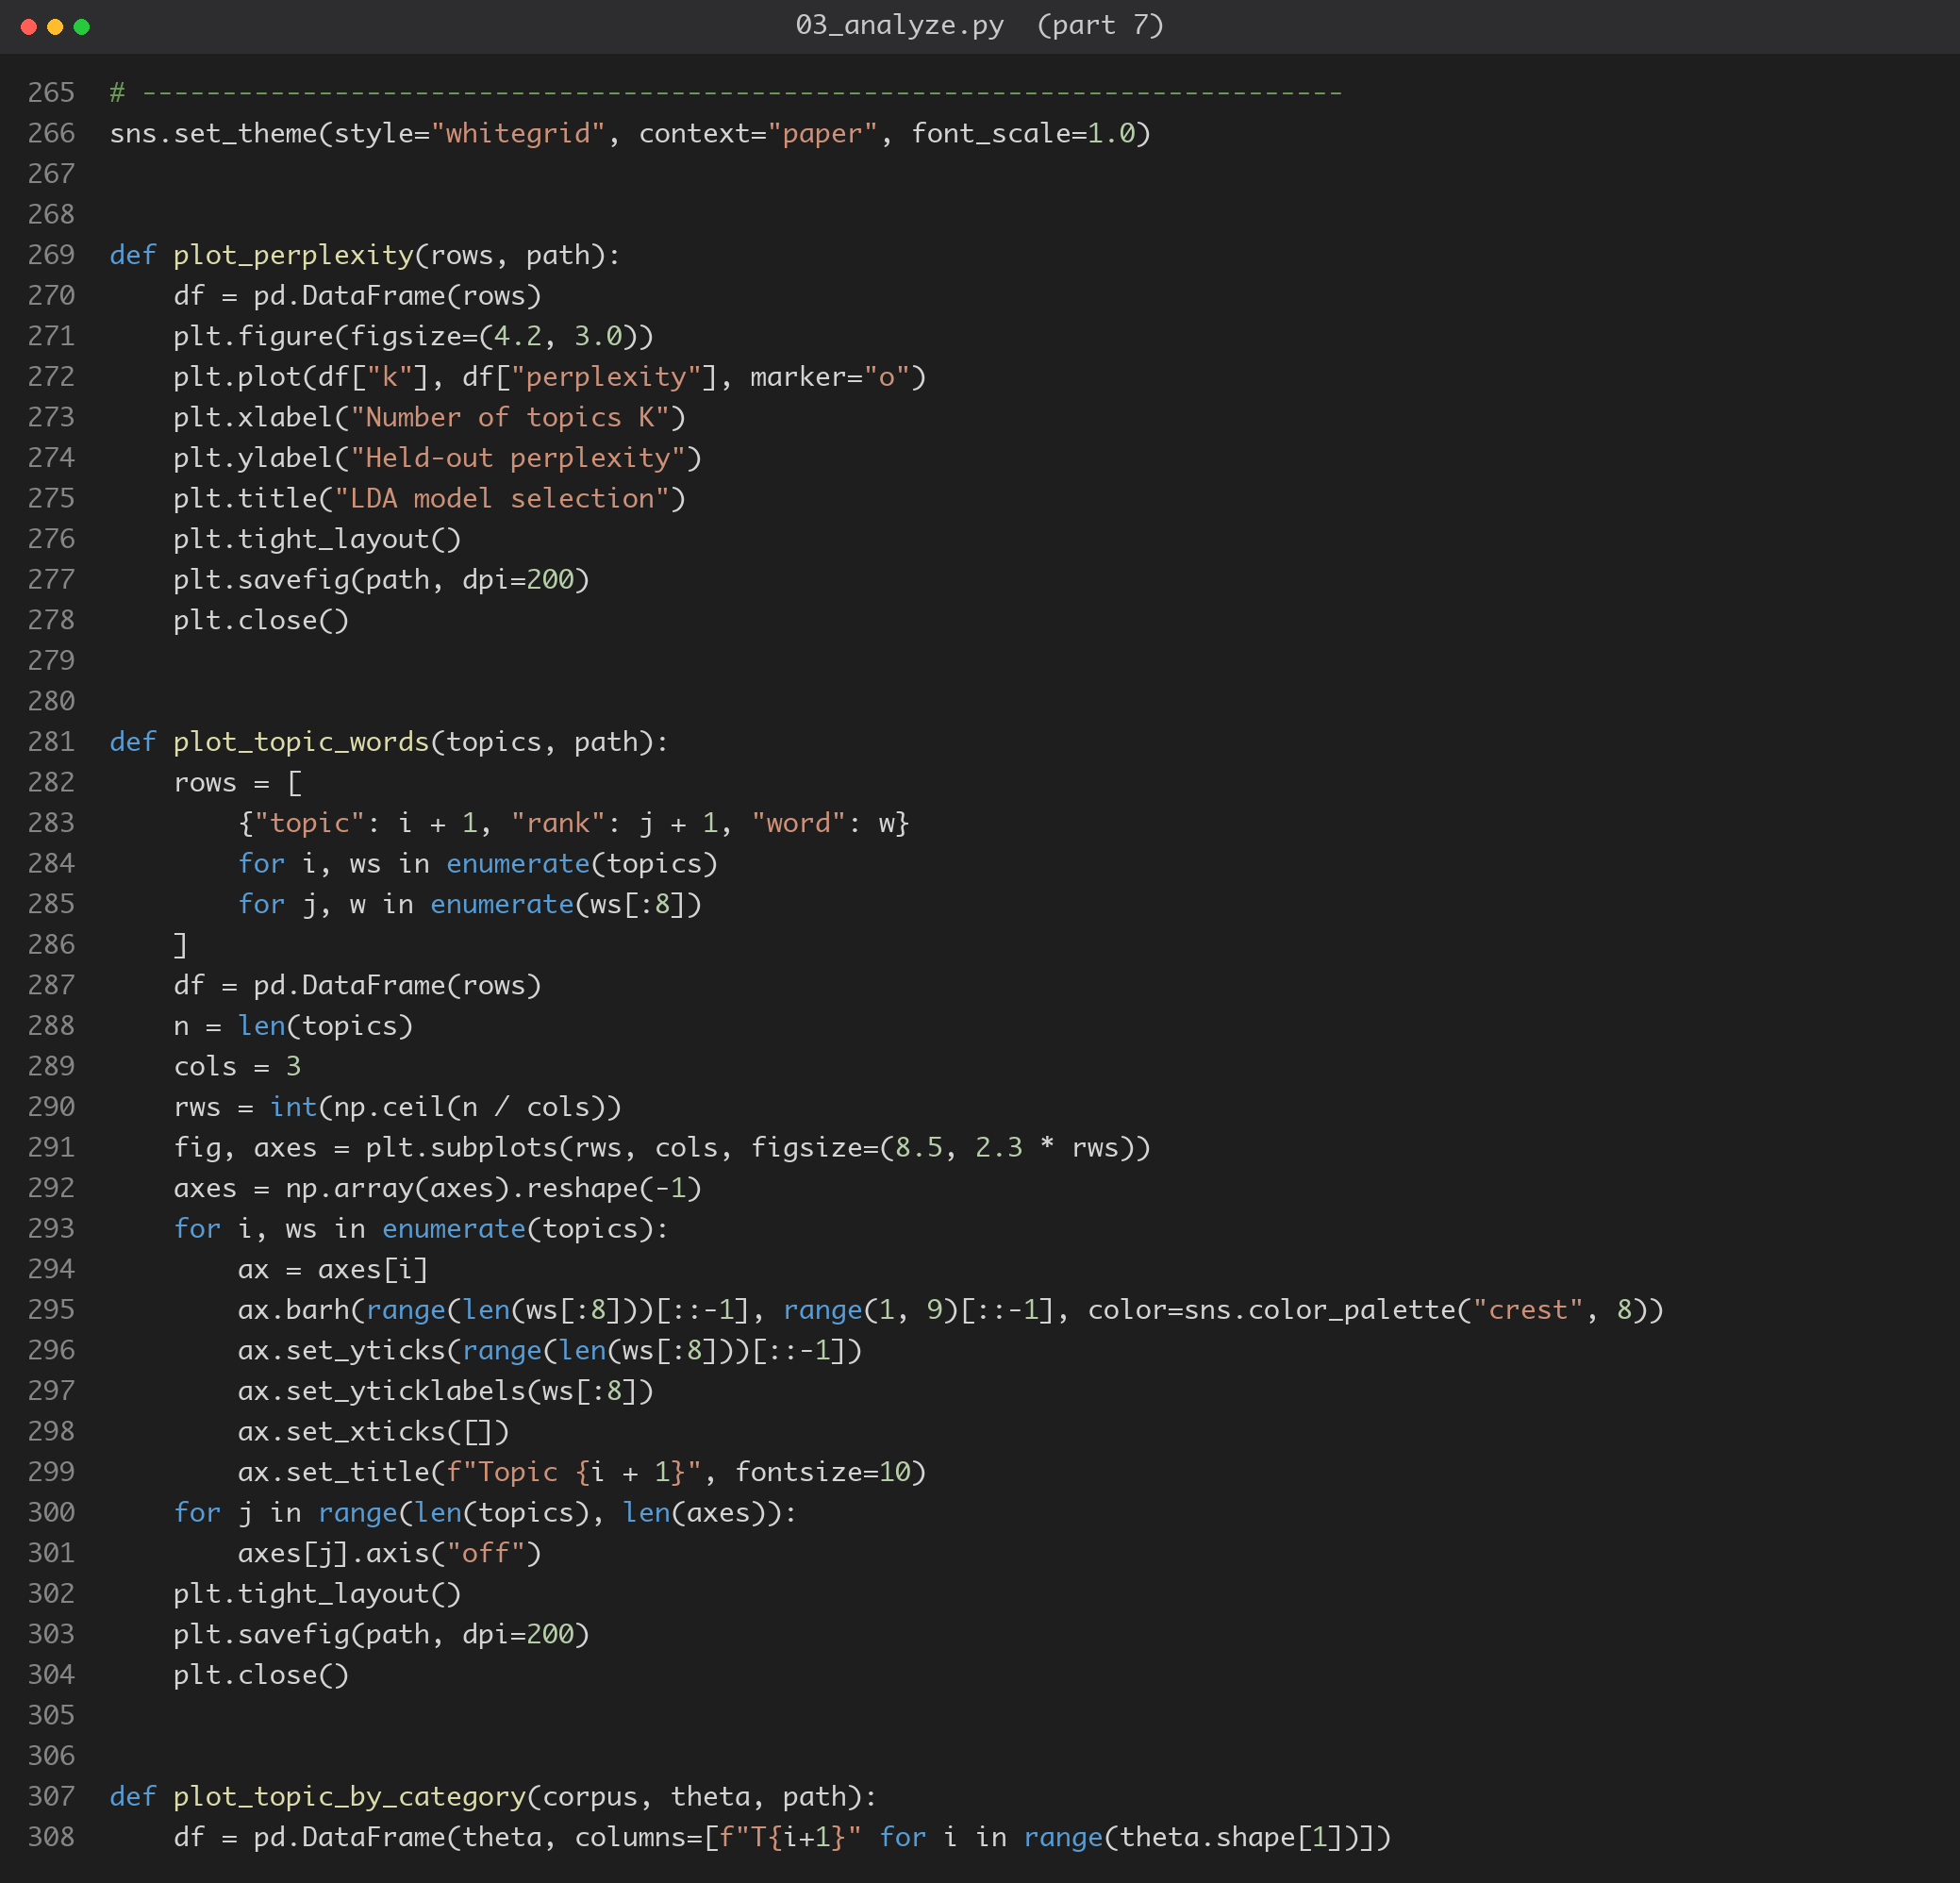
\includegraphics[width=\linewidth]{code_shots/03_analyze_py_p7.png}
\par\medskip\noindent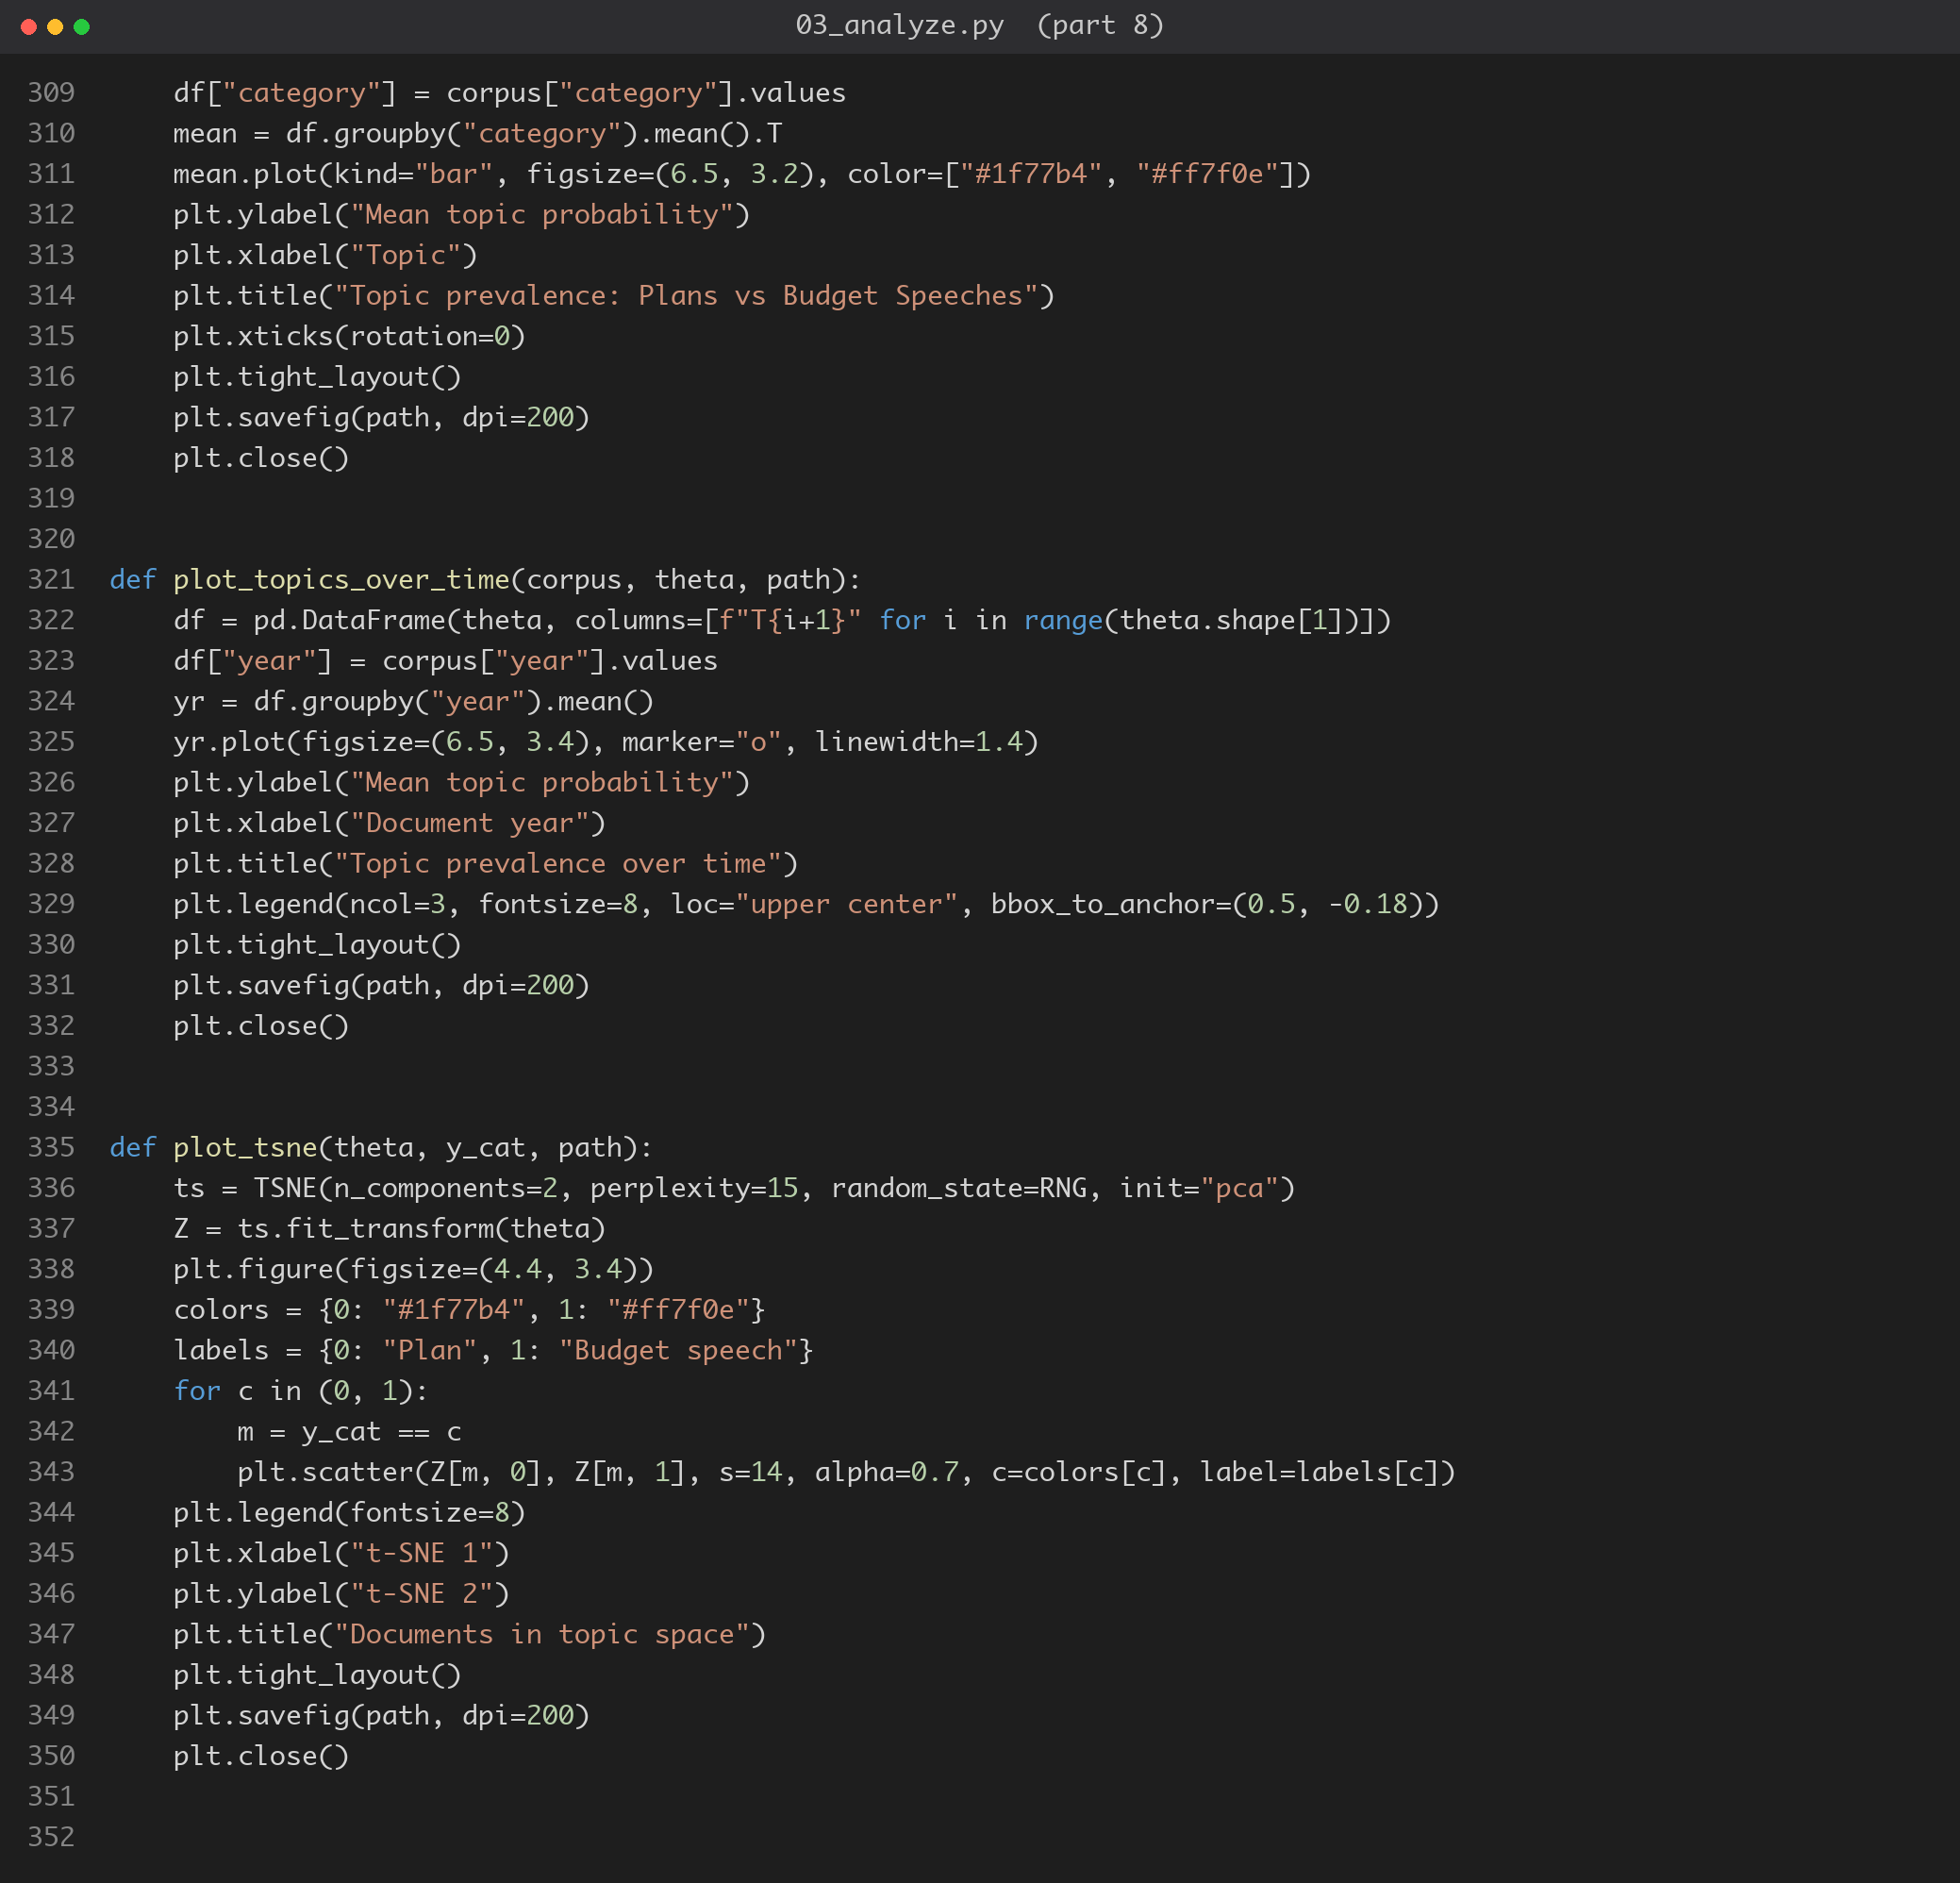
\includegraphics[width=\linewidth]{code_shots/03_analyze_py_p8.png}
\par\medskip\noindent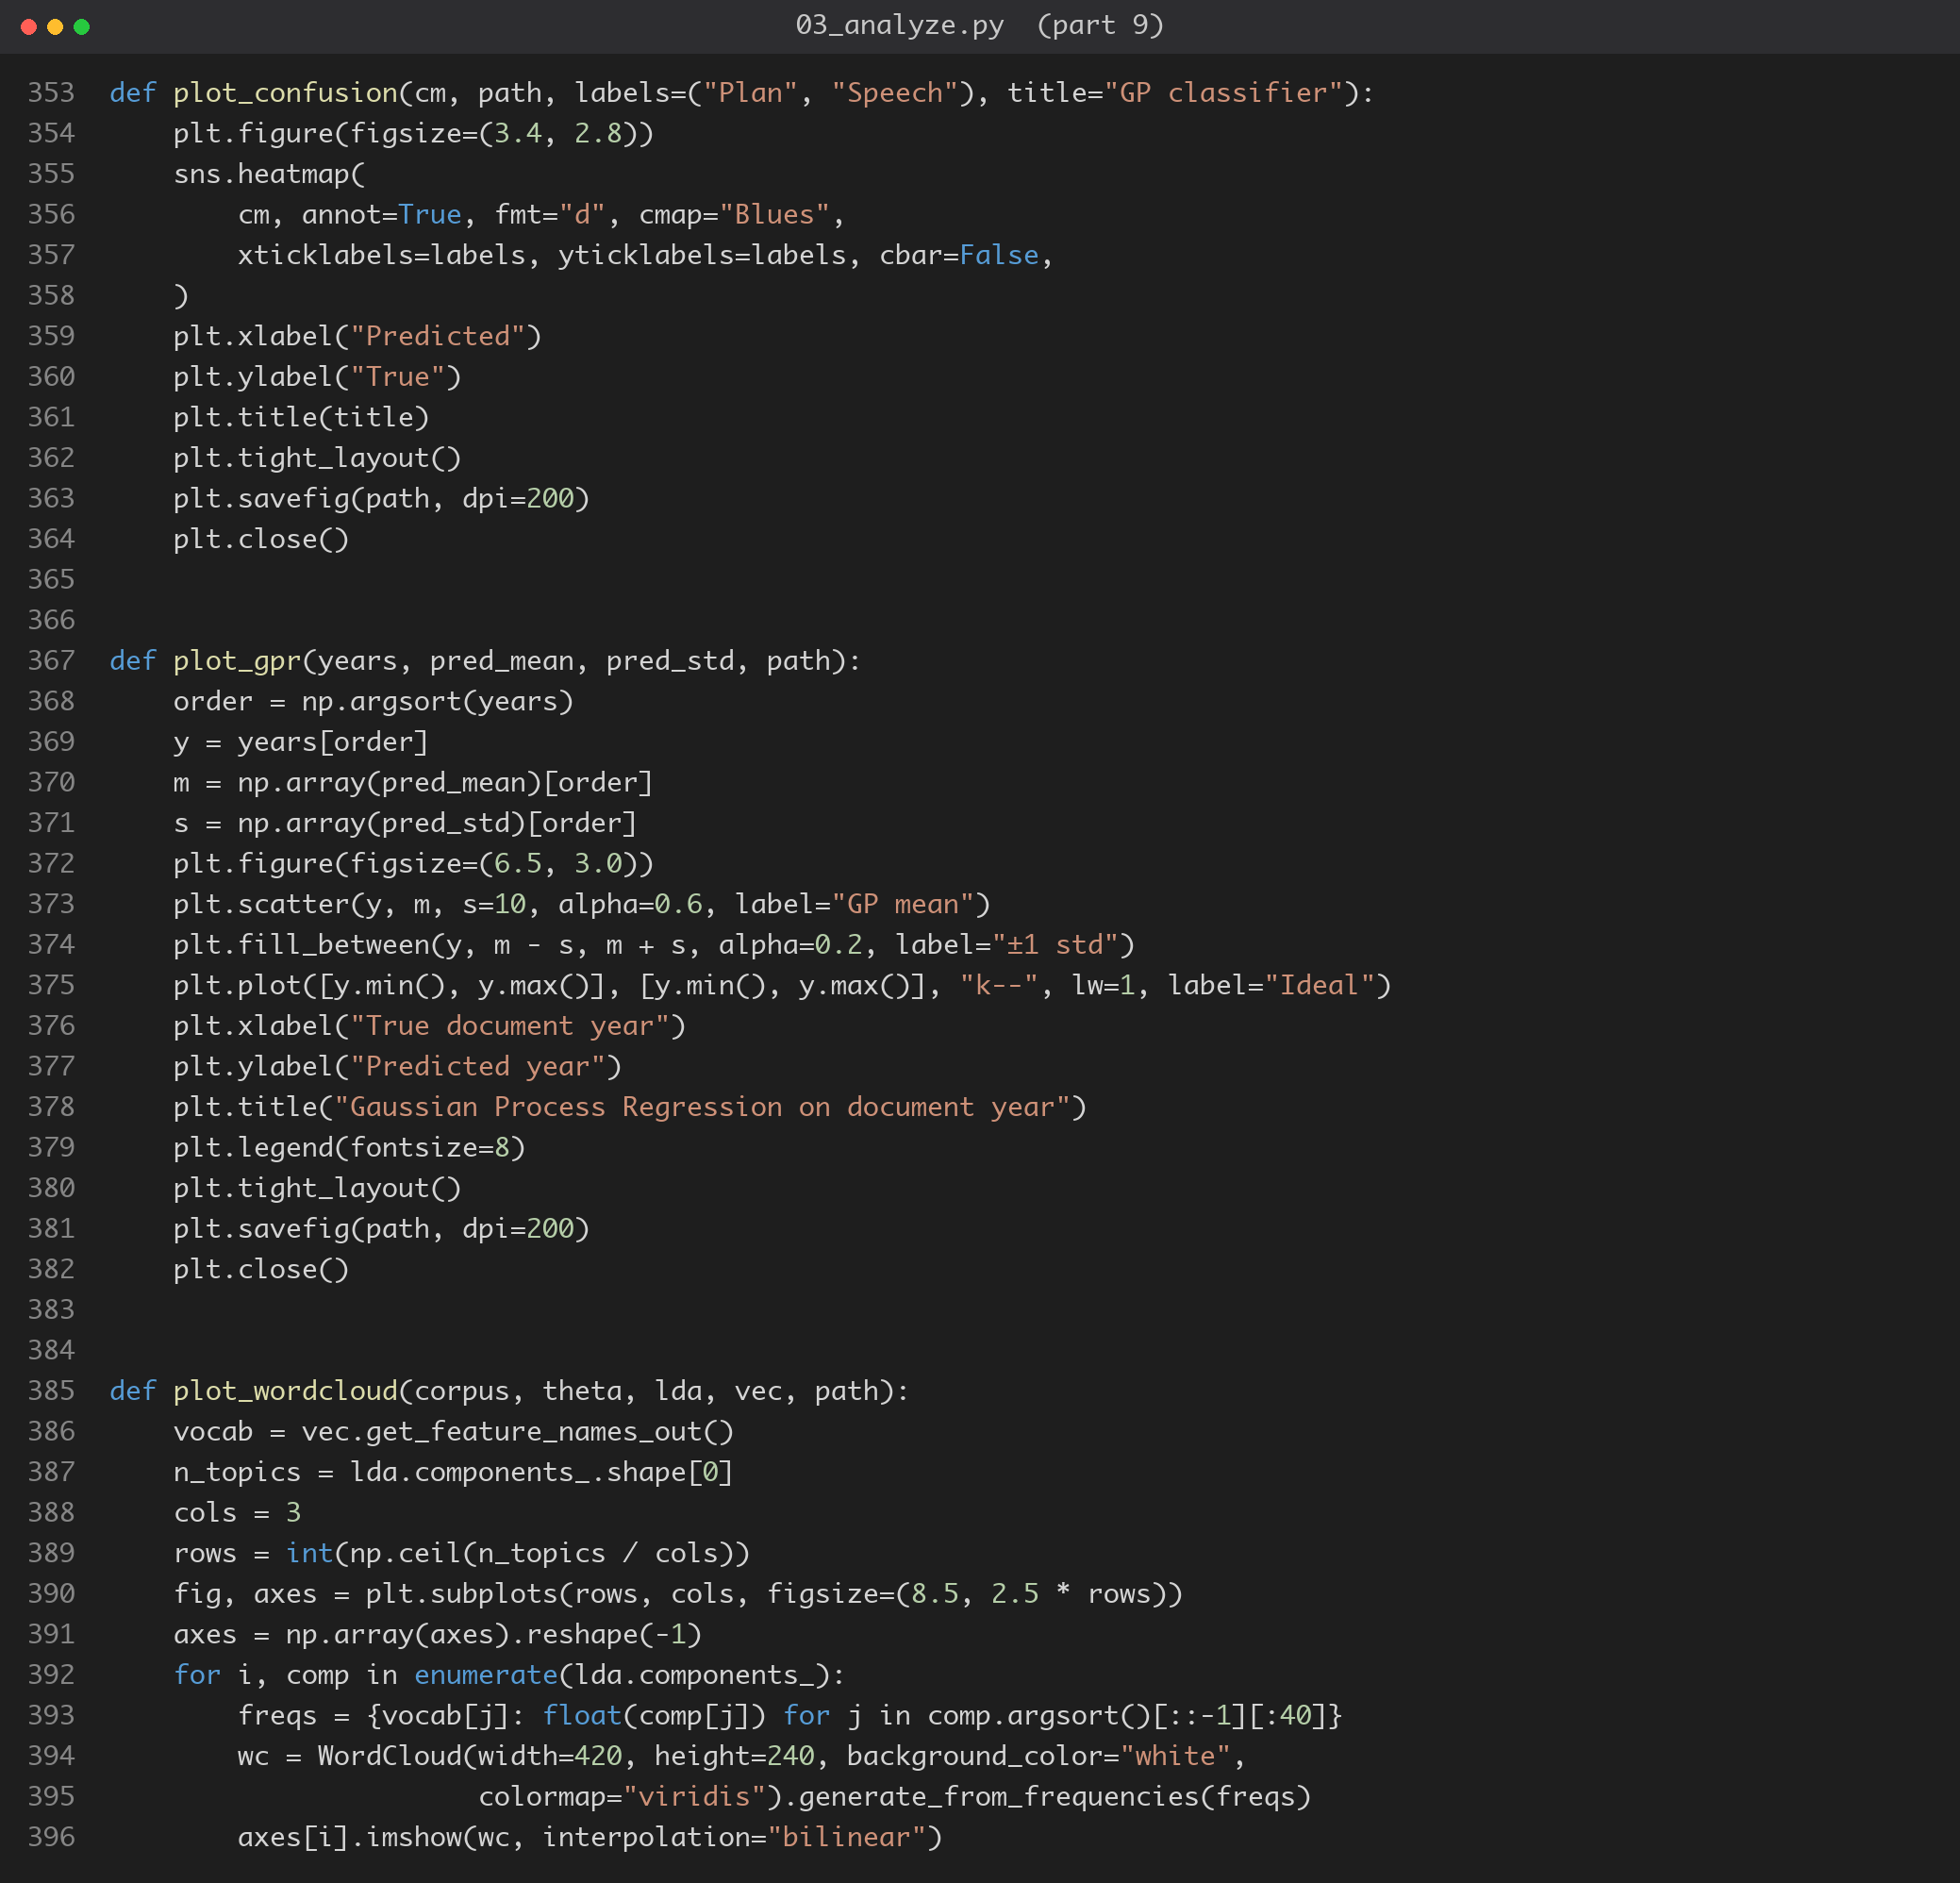
\includegraphics[width=\linewidth]{code_shots/03_analyze_py_p9.png}
\par\medskip\noindent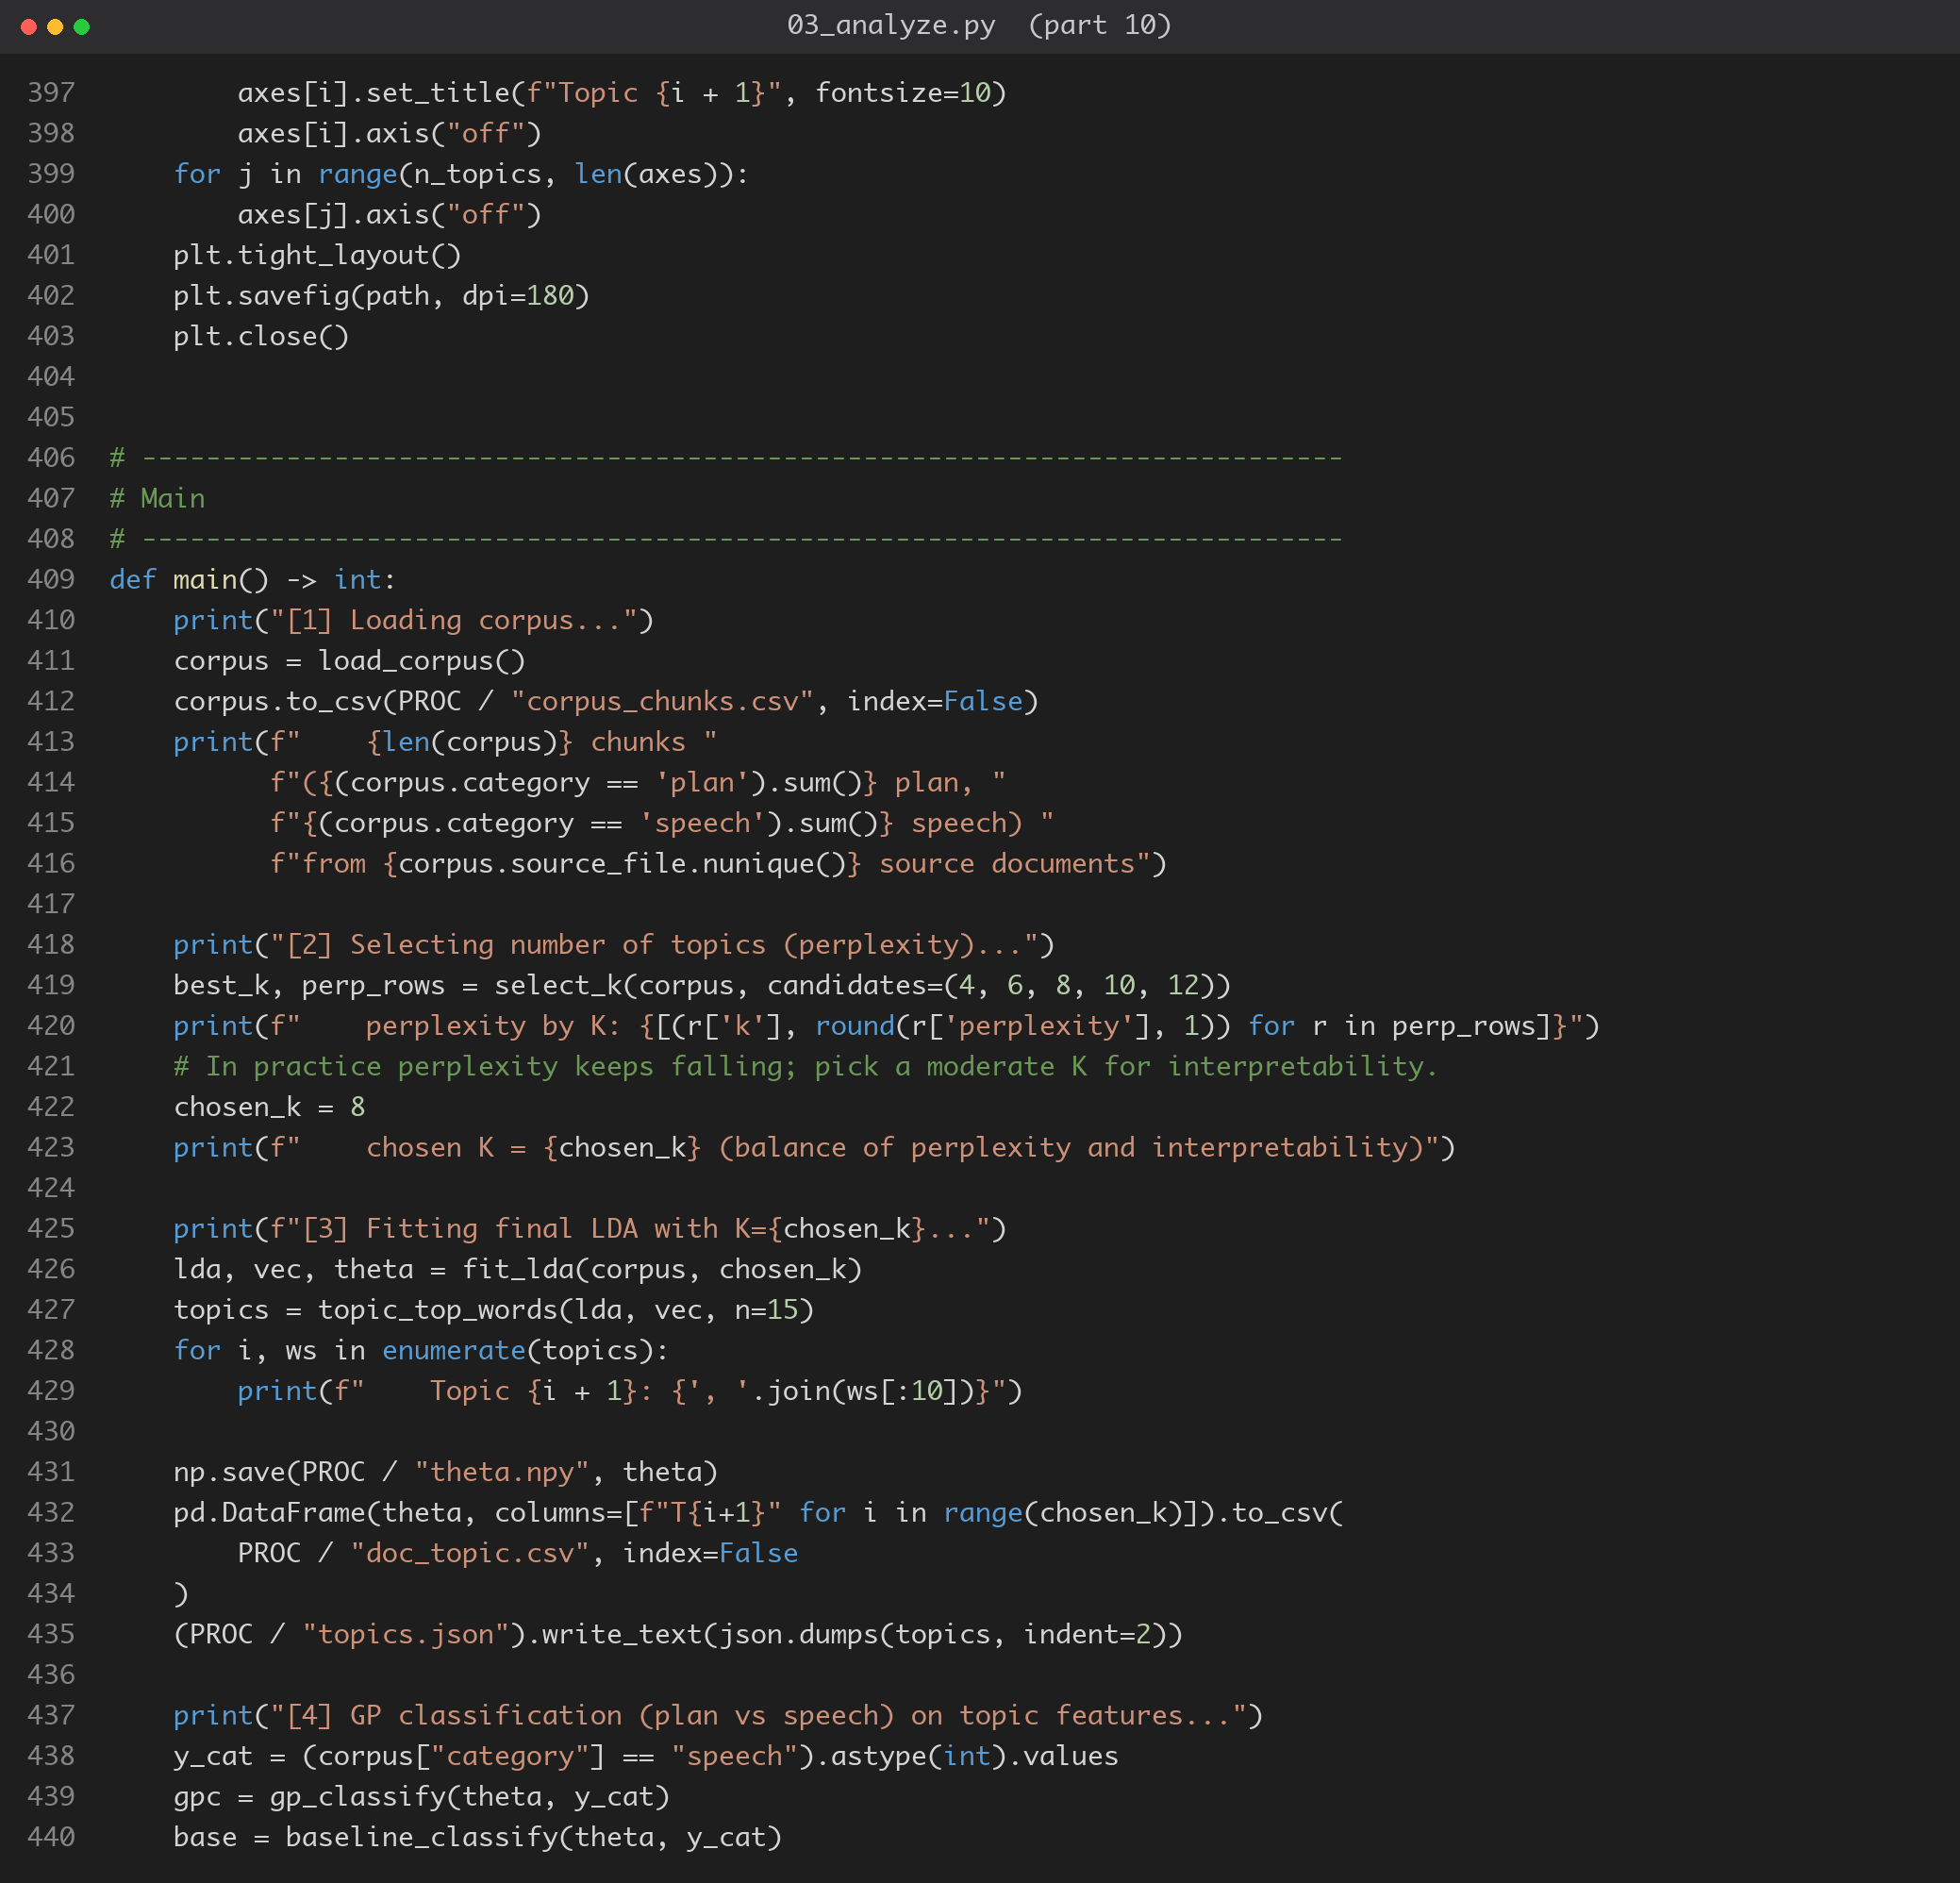
\includegraphics[width=\linewidth]{code_shots/03_analyze_py_p10.png}
\par\medskip\noindent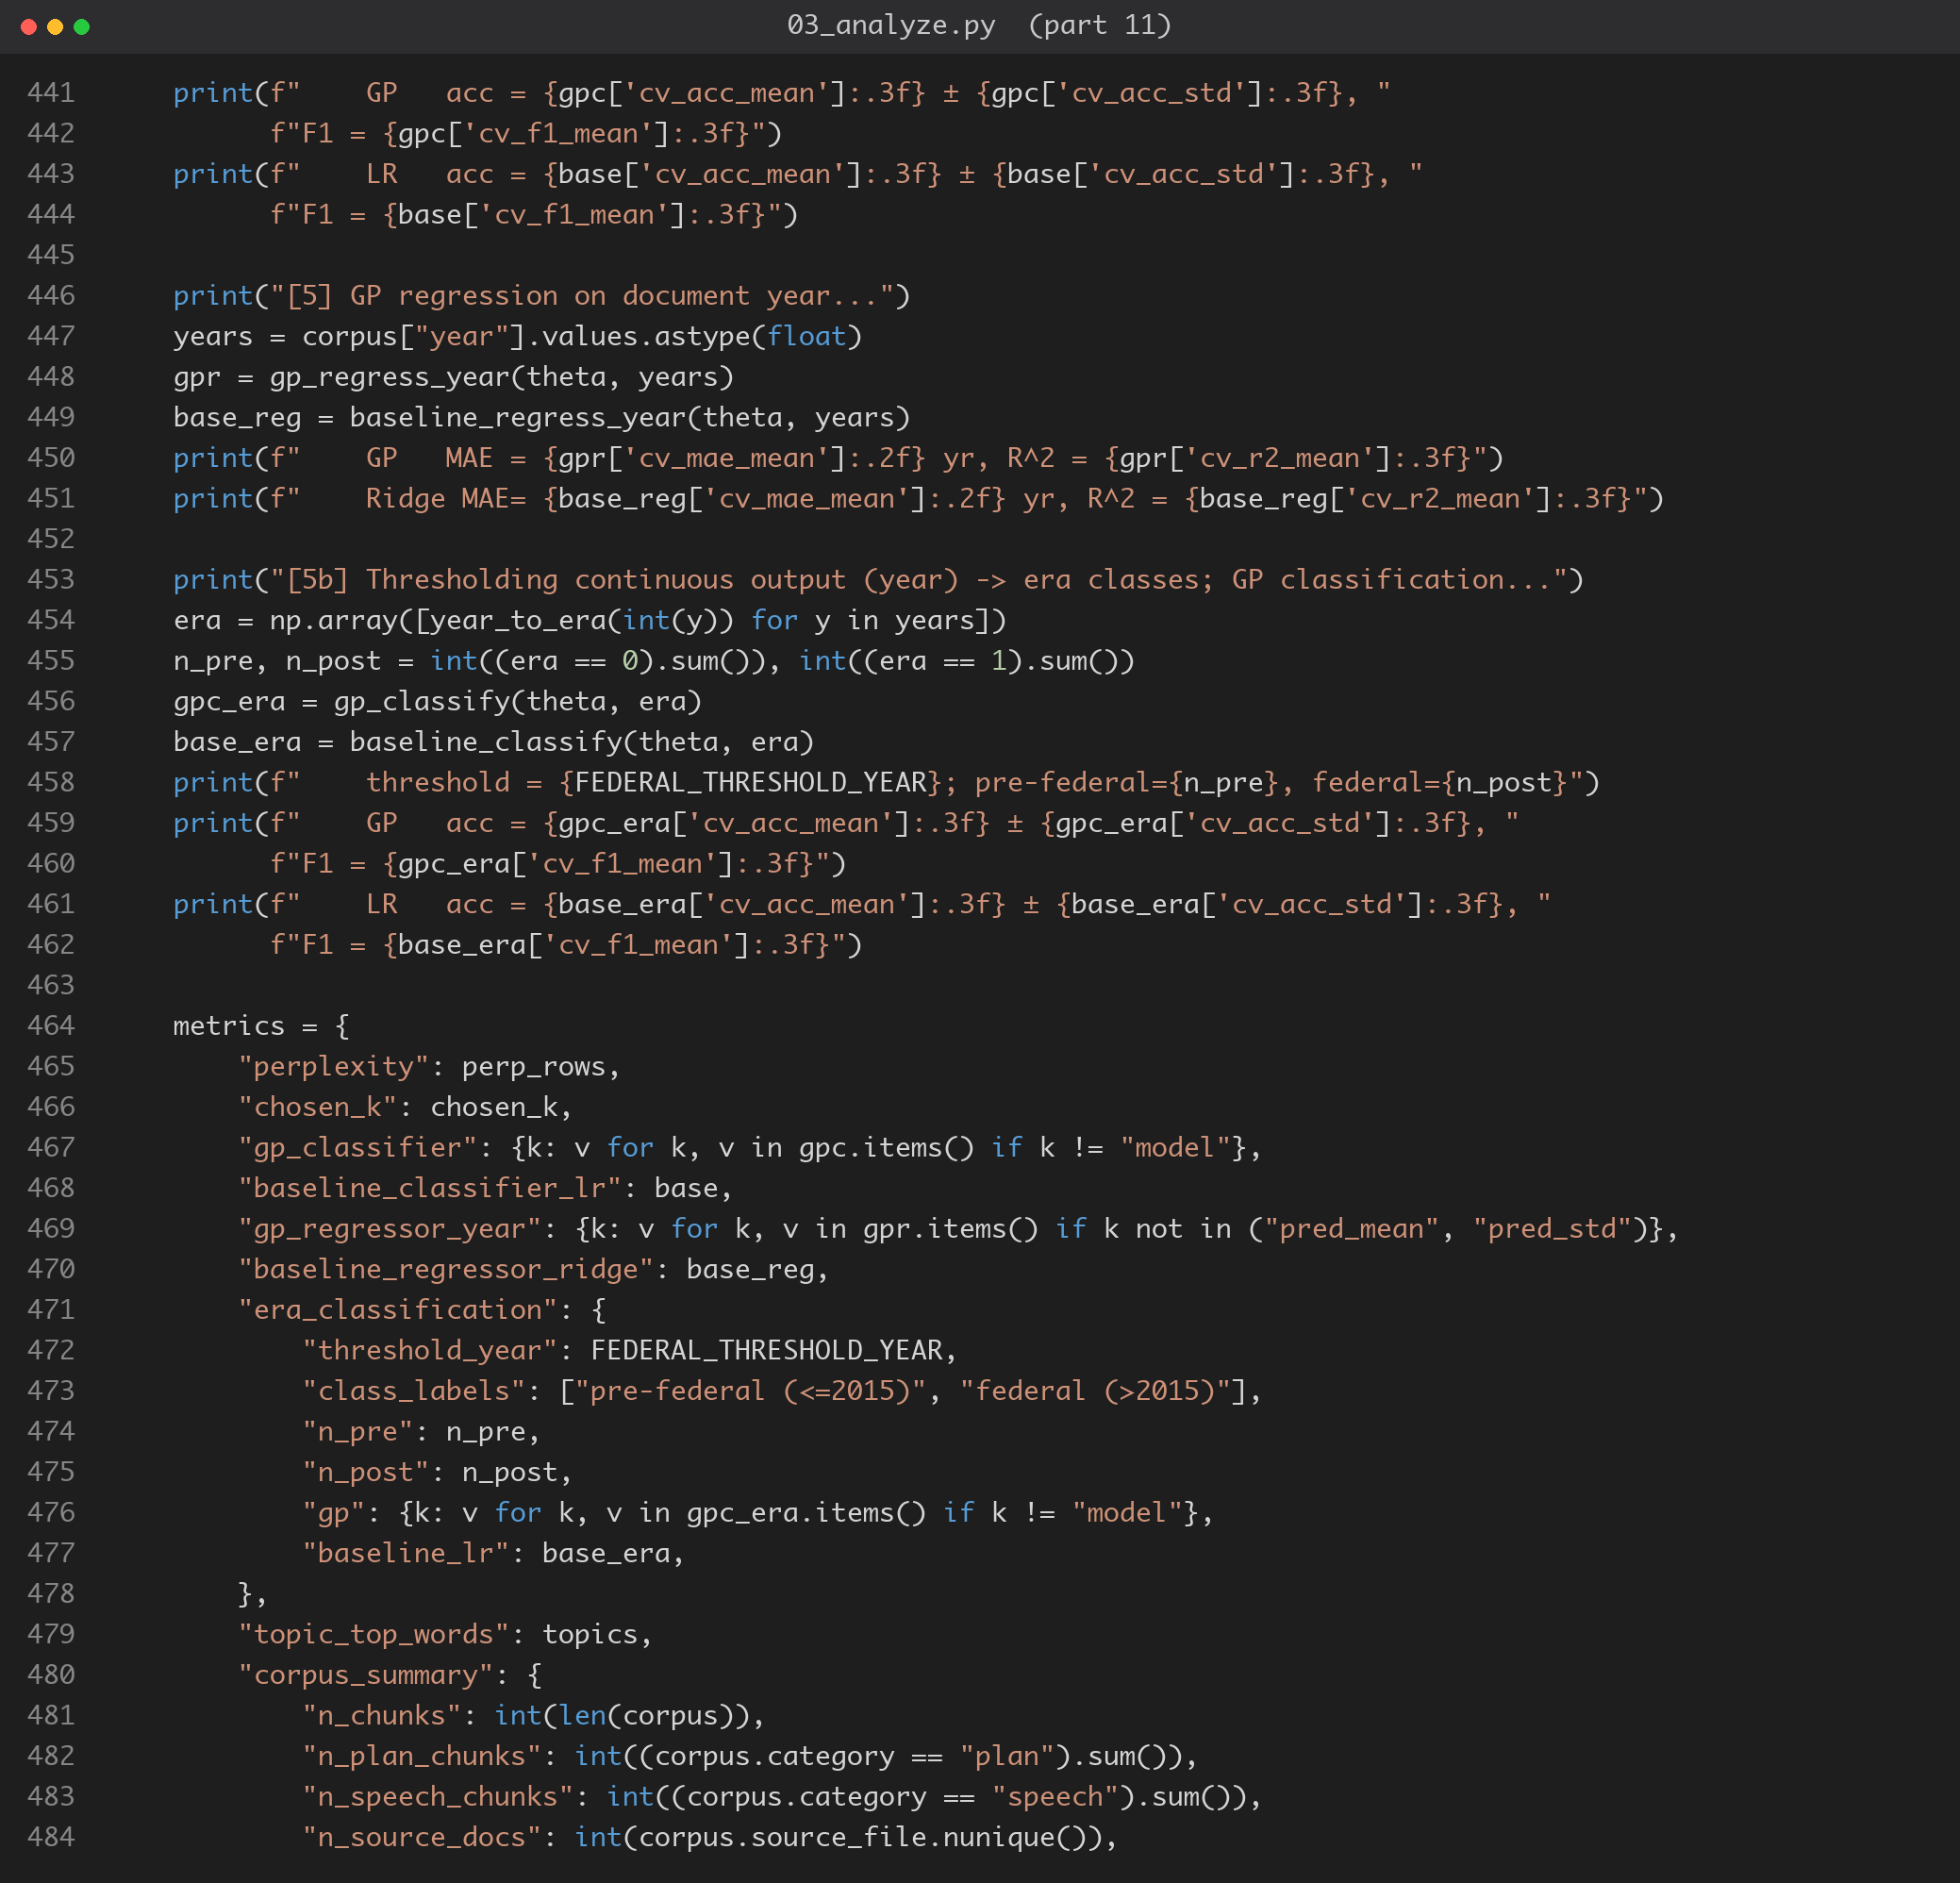
\includegraphics[width=\linewidth]{code_shots/03_analyze_py_p11.png}
\par\medskip\noindent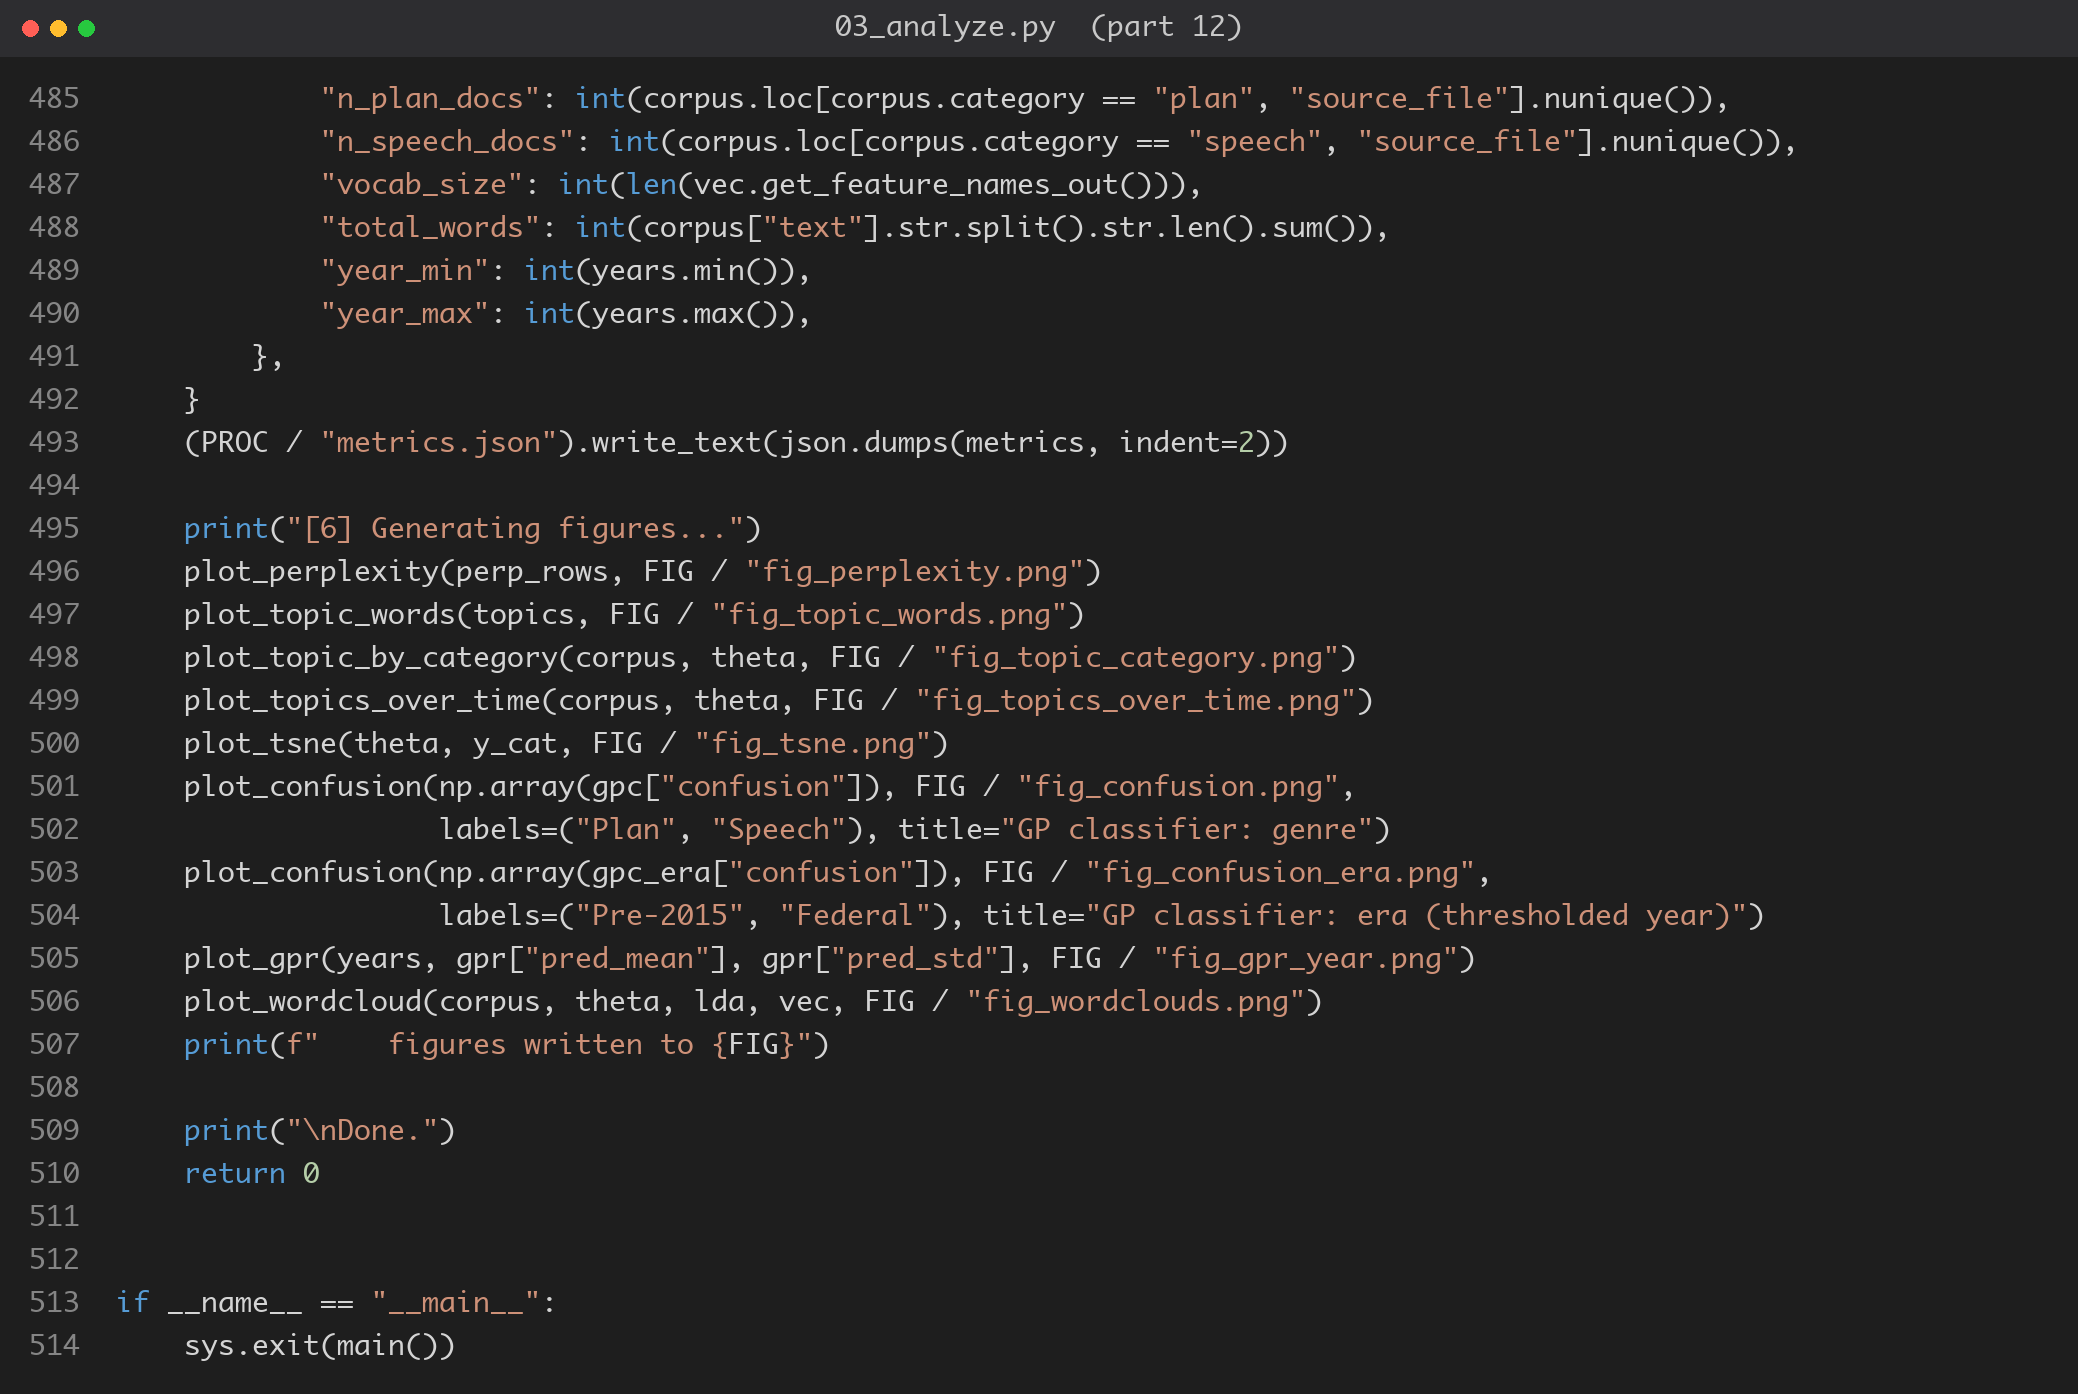
\includegraphics[width=\linewidth]{code_shots/03_analyze_py_p12.png}

\end{document}
